% Created 2017-10-27 Fr 15:36
% Intended LaTeX compiler: pdflatex
\documentclass[11pt]{article}
\usepackage[utf8]{inputenc}
\usepackage[T1]{fontenc}
\usepackage{graphicx}
\usepackage{grffile}
\usepackage{longtable}
\usepackage{wrapfig}
\usepackage{rotating}
\usepackage[normalem]{ulem}
\usepackage{amsmath}
\usepackage{textcomp}
\usepackage{amssymb}
\usepackage{capt-of}
\usepackage{hyperref}
\author{Marvin Johanning}
\date{\today}
\title{Spacemacs documentation}
\hypersetup{
 pdfauthor={Marvin Johanning},
 pdftitle={Spacemacs documentation},
 pdfkeywords={},
 pdfsubject={},
 pdfcreator={Emacs 25.3.1 (Org mode 9.1.2)}, 
 pdflang={English}}
\begin{document}

\maketitle
\tableofcontents


\section{Core Pillars}
\label{sec:org8c6bcc7}
Four core pillars: Mnemonic, Discoverable, Consistent and "Crowd-Configured".

If any of these core pillars is violated open an issue and we'll try our best
to fix it.

\subsection{Mnemonic}
\label{sec:org830ebda}
Key bindings are organized using mnemonic prefixes like \texttt{b} for buffer, \texttt{p} for
project, \texttt{s} for search, \texttt{h} for help, etc\ldots{}

\subsection{Discoverable}
\label{sec:org7504347}
Innovative real-time display of available key bindings. Simple query
system to quickly find available layers, packages, and more.

\subsection{Consistent}
\label{sec:org20f9f8b}
Similar functionalities have the same key binding everywhere thanks to a
clearly defined set of conventions. Documentation is mandatory for any layer
that ships with Spacemacs.

\subsection{Crowd-Configured}
\label{sec:orgb1da6fa}
Community-driven configuration provides curated packages tuned by power users
and bugs are fixed quickly.

\section{Highlighted feature}
\label{sec:org7d7c6bd}
\begin{itemize}
\item \textbf{Bring the efficiency of modal editing} to the powerful Emacs lisp platform.
Modal UX is optional and Spacemacs can be used with only Emacs key bindings.

\item Integrate nicely with \texttt{Evil} states (\texttt{Vim} modes).

\item \textbf{Keep your fingers on the home row} for quicker editing with support for
QWERTY and BEPO layouts.

\item \textbf{Minimalistic and nice graphical UI} keeps your available screen space for
what matters: your text files.

\item \textbf{Fast boot time}: packages and configuration are lazy-loaded as much as
possible.

\item \textbf{Lower the risk of RSI} by heavily using the space bar instead of modifiers.
If you have issues with your thumbs you can still use Spacemacs using
modifiers.

\item Contribute easily your improvements and new configuration layers.

\item \textbf{Very active and helpful community} on \texttt{Gitter} and \texttt{IRC}
(via Gitter IRC bridge)
\end{itemize}

\section{Screenshots}
\label{sec:orgda076db}

\begin{center}
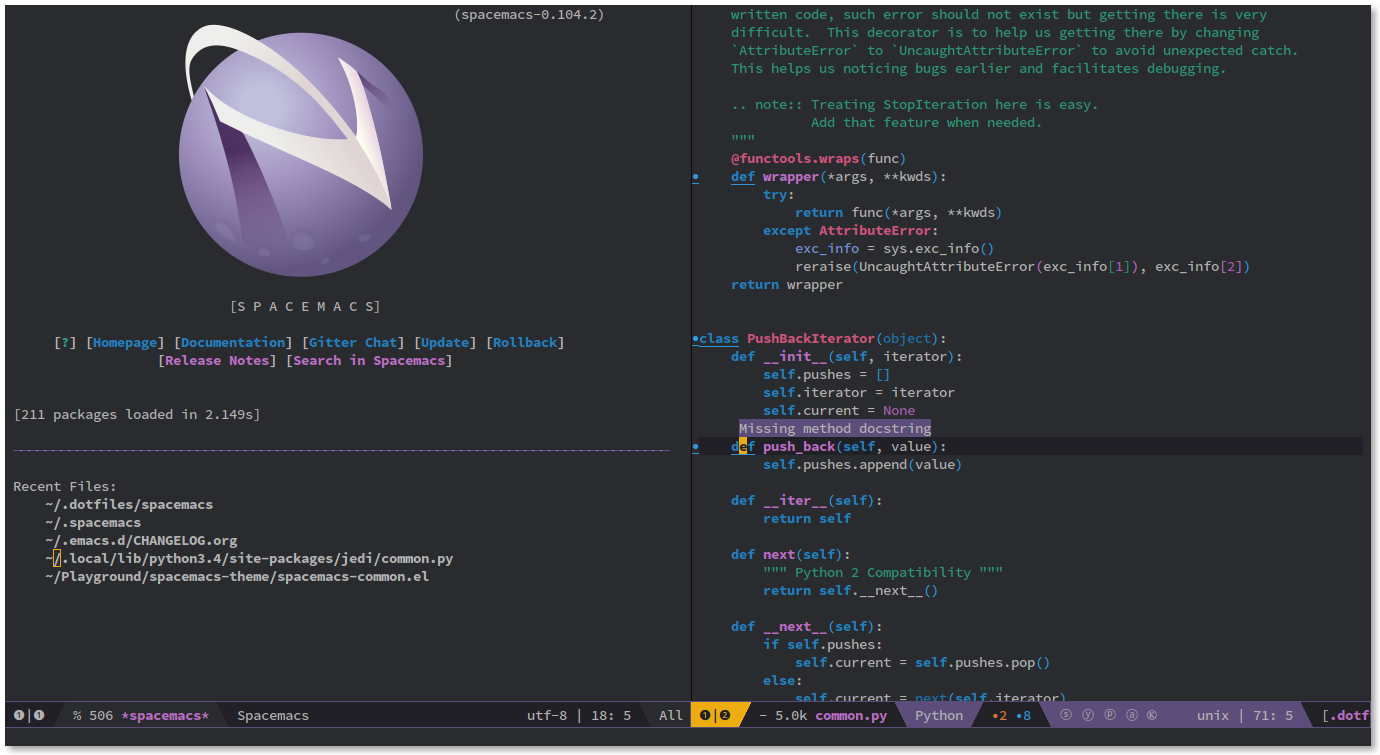
\includegraphics[width=.9\linewidth]{img/spacemacs-python.png}
\end{center}
\emph{Python}

\textbf{Note}: Even though screenshots are updated frequently, Spacemacs is evolving
quickly and the screenshots may not reflect exactly the current state of the
project.

\section{Who can benefit from this?}
\label{sec:orgc314219}
\begin{itemize}
\item Spacemacs was initially intended to be used by \textbf{Vim users} who want to go to
the next level by using Emacs (see \href{VIMUSERS.org}{guide} for Vimmers). But it is now
perfectly \textbf{usable by non Vim users} by choosing the \texttt{emacs} editing style.

\item It is also a good fit for people wanting to \textbf{lower the \href{http://en.wikipedia.org/wiki/Repetitive\_strain\_injury}{risk of RSI}} induced by
the default Emacs key bindings. (This is an assumption, there are no official
studies to prove this!) If you have issues using your thumbs you can still
use the \texttt{emacs} editing style which puts the leader key on a modifier
combination.

\item Emacs users wanting to learn \textbf{a different way to edit files} or wanting to
learn Vim key bindings or even wanting to mix both editing styles by setting
their style to \texttt{hybrid}.

\item Emacs users wanting a simple but deep configuration system that greatly
\textbf{lower the risk of .emacs bankruptcy}.

\item \textbf{Pair-programming} users thanks to out of the box support for dynamic
switching of editing style. A Vim user and an Emacs user can use the same
Spacemacs comfortably.
\end{itemize}

\section{Update and Rollback}
\label{sec:org07a4b7a}
\subsection{Update Spacemacs repository}
\label{sec:org4b00a0b}
There are several methods of updating the core files and layer information for
Spacemacs. It is recommended to update the packages first; see the next section.

\subsubsection{Automatic Updates}
\label{sec:org63c649f}
Spacemacs will automatically check for a new version every startup. When it
detects that a new version is available an arrow will appear in the modeline.
Click it to update Spacemacs. You must restart Emacs after updating.
\begin{center}
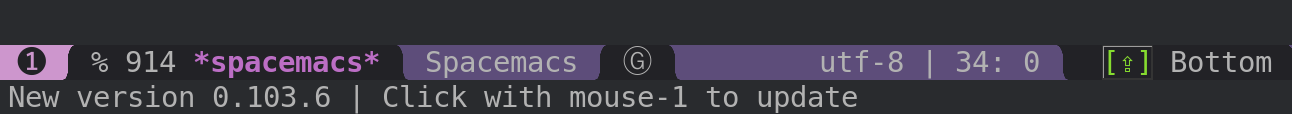
\includegraphics[width=.9\linewidth]{img/powerline-update.png}
\end{center}
\emph{Update Button}

\textbf{Note}: If you use the \texttt{develop} branch of Spacemacs, automatic update is
disabled---you have to update manually using git.

\subsubsection{Updating from the Spacemacs Buffer}
\label{sec:orgb2e603f}
Use the button labeled "Update Spacemacs" in the Spacemacs buffer. You will be
prompted for the version you would like to use.

\textbf{Note}: If you use the \texttt{develop} branch of Spacemacs, you cannot use this method.

\subsubsection{Updating Manually with git}
\label{sec:org40264be}
To update manually close Emacs and update the git repository:

\begin{verbatim}
$ git pull origin master
\end{verbatim}

\textbf{Note}: The master branch is considered to be immutable in the sense that you
must not modify it by adding your own commit. If you do so you will break the
automatic update of Spacemacs on the master branch. To fork Spacemacs code you
have to use a custom branch that you manage manually.

\subsection{Update packages}
\label{sec:org23706c6}
To update the Emacs packages used by Spacemacs press RET (enter) or click on the
link \texttt{[Update Packages]} in the startup page under the banner then restart
Emacs. If you prefer, you can use the command
\texttt{configuration-layer/update-packages} instead of the button.

If anything goes wrong you should be able to rollback the update by pressing
\texttt{RET} or clicking on the \texttt{[Rollback Package Update]} link in the startup page
and choosing a rollback slot (sorted by date). This button uses the command
\texttt{configuration-layer/rollback}.

\section{Configuration layers}
\label{sec:org5007336}
This section is an overview of layers. A more extensive introduction to writing
configuration layers can be found \href{LAYERS.org}{here} (recommended reading!).

\subsection{Purpose}
\label{sec:orgc9d1819}
Layers help collect related packages together to provide features. For example,
the \texttt{python} layer provides auto-completion, syntax checking, and REPL support
for python files. This approach helps keep configuration organized and reduces
overhead for the user by keeping them from having to think about what packages
to install. To install all the \texttt{python} features the user has just to add the
\texttt{python} layer to their dotfile.

\subsection{Structure}
\label{sec:orgc1287dc}
Configuration is organized in layers. Each layer has the following structure:

\begin{verbatim}
[layer_name]
  |__ [local]
  | |__ [package 1]
  | |     ...
  | |__ [package n]
  |-- layers.el
  |__ packages.el
  |__ funcs.el
  |__ config.el
  |__ keybindings.el

[] = directory
\end{verbatim}

Where:

\begin{center}
\begin{tabular}{ll}
File & Usage\\
\hline
layers.el & The place to declare additional layers\\
packages.el & The list of packages and their configuration functions (init, post-init, etc\ldots{})\\
funcs.el & All functions defined in the layer (used in package configuration for instance)\\
config.el & Layer configuration (defines the layer variables default values and setup some config variables)\\
keybindings.el & General key bindings no tied to a specific package configuration\\
\end{tabular}
\end{center}

\texttt{Packages} can be:
\begin{itemize}
\item \texttt{ELPA} packages installed from an \texttt{ELPA} compliant repository
\item local packages in a layer's \texttt{local} folder
\item installed from an online source using \href{https://github.com/quelpa/quelpa}{quelpa}.
\end{itemize}

\subsection{Configure packages}
\label{sec:orgc3529e4}
\subsubsection{With a layer}
\label{sec:org5255067}
\begin{enumerate}
\item Declaration
\label{sec:org3717d51}
\texttt{Packages} are declared in a variable called \texttt{<layer>-packages} where \texttt{<layer>}
is the name of the layer.

Example:

\begin{verbatim}
(setq <layer>-packages '(package1 package2 ...)
\end{verbatim}

All packages from all layers are processed in alphabetical order so sometimes
you'll have to use some \texttt{with-eval-after-load} black magic to configure them
properly. For instance if package \texttt{A} depends on \texttt{B} then you can configure
\texttt{A} with:

\begin{verbatim}
(with-eval-after-load 'B ...)
\end{verbatim}

For details on installing packages using quelpa or local packages see \href{LAYERS.org}{LAYERS}.

\item Initialization
\label{sec:org8df144f}
To initialize a package \texttt{xxx}, define a function with this format in
\texttt{packages.el}:

\begin{verbatim}
(defun <layer>/init-xxx () ...body )
\end{verbatim}

It is common to define the body with the \href{https://github.com/jwiegley/use-package}{use-package} macro.

\item Exclusion
\label{sec:org8fcd62b}
It is possible to exclude some packages from Spacemacs on a per-layer basis.
This is useful when a configuration layer aims to replace a stock package
declared in the Spacemacs layer.

To do so add the package names to exclude to the variable
\texttt{<layer>-excluded-packages}.

Example:

\begin{verbatim}
(setq <layer>-excluded-packages '(package1 package2 ...)
\end{verbatim}
\end{enumerate}

\subsubsection{Without a layer}
\label{sec:org89982df}
Sometimes a layer can be an unnecessary overhead, this is the case if you just
want to install a package with very few configuration associated to it. A good
example is some niche language where you are only interested in syntax
highlighting.

You can install such packages by adding them to the variable
\texttt{dotspacemacs-additional-packages} under the \texttt{dotspacemacs/layers} function in your dotfile.

For example, to install \texttt{llvm-mode} and \texttt{dts-mode}:
\begin{verbatim}
(defun dotspacemacs/layers ()
  "Configuration Layers declaration..."
  (setq-default
   ;; ...
   dotspacemacs-additional-packages '(llvm-mode dts-mode)
   ;; ...
   ))
\end{verbatim}

If you want to add some configuration for them then put the configuration in
the \texttt{dotspacemacs/user-config} function or consider creating a layer.

\subsection{Packages synchronization}
\label{sec:orgcd82dc2}
Spacemacs will only install the packages that are explicitly used by the user.
A package is considered to be used if its layer is used (i.e. listed in
\texttt{dotspacemacs-configuration-layers}).
Any packages that are not used is considered to be orphan and is deleted at
the next startup of Emacs.

\subsection{Types of configuration layers}
\label{sec:org15bae51}
There are two types of configuration layers:
\begin{itemize}
\item distributed layers (in the \texttt{layers} directory, those layers are contributions shared
by the community and merged upstream)
\item private (in the \texttt{private} directory, they are ignored by Git)
\end{itemize}

\subsection{Submitting a configuration layer upstream}
\label{sec:org64da027}
If you decide to provide a configuration layer, please check the contribution
guidelines first in \href{../CONTRIBUTING.org}{CONTRIBUTING}.

\subsection{Example: Themes Megapack example}
\label{sec:org9426a77}
This is a simple configuration layer listing a bunch of themes which you can
find \href{../layers/+themes/themes-megapack/README.org}{here}.

To install it, just add \texttt{themes-megapack} to your \texttt{\textasciitilde{}/.spacemacs} like so:

\begin{verbatim}
(setq-default dotspacemacs-configuration-layers '(themes-megapack))
\end{verbatim}

Adding this layer will install around 100 themes; to uninstall them remove the
layer from the \texttt{dotspacemacs-configuration-layers} and press \texttt{SPC f e R}.

\subsection{Managing private configuration layers}
\label{sec:orgba0847d}
Spacemacs's configuration system is flexible enough to let you manage your
private layers in different ways.

\subsubsection{Using the private directory}
\label{sec:orgf3c7a51}
Everything in the private directory is ignored by Git so it is a good place to
store private layers. There is a huge drawback to this approach though: \emph{your
layers are not source controlled}.

\subsubsection{Using an external Git repository}
\label{sec:org25eccaa}
This is the recommended way to manage your private layers.

The best approach is to store all your private layers into an external Git
repository. It is especially a good practice to store them in your \texttt{dotfiles}
repository if you have one. Put also your \texttt{\textasciitilde{}/.spacemacs} file in it.

Then you are free to symlink your layers into \texttt{\textasciitilde{}/emacs.d/private} \emph{or} let them
anywhere you want and reference the parent directory in the variable
\texttt{dotspacemacs-configuration-layer-path} of your \texttt{\textasciitilde{}/.spacemacs}.

Note that you could also have a dedicated repository for all your private layers
and then directly clone this repository in \texttt{\textasciitilde{}/.emacs.d/private}.

\subsubsection{Using a personal branch}
\label{sec:org6ca380e}
The final main way to manage your private layers is to push them in a personal
branch that you keep up to date with upstream \texttt{master} or \texttt{develop}.

\subsection{Tips for writing layers}
\label{sec:org774f04d}
Please refer to \href{LAYERS.org}{this} introduction for some tips on writing layers, and how to
best make them fit with the Spacemacs philosophy and loading strategy.

\section{Dotfile Configuration}
\label{sec:org716eb74}
User configuration can be stored in your \texttt{\textasciitilde{}/.spacemacs} file.

\subsection{Dotfile Installation}
\label{sec:org8b54f23}
The very first time Spacemacs starts up, it will ask you several questions
and then install the \texttt{.spacemacs} in your \texttt{HOME} directory.

\subsection{Alternative dotdirectory}
\label{sec:org358209a}
A dotdirectory \texttt{\textasciitilde{}/.spacemacs.d/} can be used instead of a dotfile.
If you want to use this option, move \texttt{\textasciitilde{}/.spacemacs} to \texttt{\textasciitilde{}/.spacemacs.d/init.el}.

It is also possible to override the location of \texttt{\textasciitilde{}/.spacemacs.d/} using the
environment variable \texttt{SPACEMACSDIR}. Of course you can also use symlinks to
change the location of this directory.

\textbf{Note:} \texttt{\textasciitilde{}/.spacemacs} will always take priority over \texttt{\textasciitilde{}/.spacemacs.d/init.el},
so \texttt{\textasciitilde{}/.spacemacs} must not exist for \texttt{\textasciitilde{}/.spacemacs.d/init.el} to be used by
Spacemacs.

\subsection{Synchronization of dotfile changes}
\label{sec:org3605dd6}
To apply the modifications made in \texttt{\textasciitilde{}/.spacemacs} press \texttt{SPC f e R}. It will
re-execute the Spacemacs initialization process.

\textbf{Note}: A synchronization re-executes the functions \texttt{dotspacemacs/init},
\texttt{dotspacemacs/user-init} and \texttt{dotspacemacs/user-config}.
Depending on the content of this functions you may encounter some unwanted side
effects. For instance if you use a toggle in \texttt{dotspacemac/user-config} to enable
some behavior, this behavior will be turned off whenever the dotfile is
re-synchronized. To avoid these side-effects it is recommended to either use
\texttt{setq} expressions instead of toggle functions, or to use the \texttt{on} or \texttt{off}
versions instead (i.e. instead of \texttt{spacemacs/toggle-<thing>}, use
\texttt{spacemacs/toggle-<thing>-on} or \texttt{spacemacs/toggle-<thing>-off}).

It is possible to \emph{skip} the execution of \texttt{dotspacemacs/user-config} with the
universal argument (\texttt{SPC u SPC f e R}).

\subsection{Testing the dotfile}
\label{sec:orge4dded9}
You can use the command \texttt{SPC SPC dotspacemacs/test-dotfile} to check if your
\texttt{\textasciitilde{}/.spacemacs} looks correct. This will check, among other things, whether the
declared layers can be found and that the variables have sensible values. These
tests are also run automatically when you synchronize with \texttt{SPC f e R}.

\subsection{Dotfile Contents}
\label{sec:orge477d8f}
\subsubsection{Configuration functions}
\label{sec:orga3302d3}
Three special functions in the \texttt{\textasciitilde{}/.spacemacs} file can be used to perform
configuration at the beginning and end of Spacemacs loading process:

\begin{itemize}
\item \texttt{dotspacemacs/layers} is called at the very startup of Spacemacs initilialization,
this is where you set the Spacemacs distribution and declare layers to be used
in your configuration. You can also add or excluded packages of your choice
and tweak some behavior of Spacemacs loading.
\item \texttt{dotspacemacs/init} is called at the very startup of Spacemacs initialization
before layers configuration. \textbf{You should not put any user code} in there
besides modifying the Spacemacs variable values prefixed with \texttt{dotspacemacs-}.
\item \texttt{dotspacemacs/user-init} is called immediately after \texttt{dotspacemacs/init},
before layer configuration. This function is mostly useful for variables
that need to be set before packages are loaded.
\item \texttt{dotspacemacs/user-config} is called at the very end of Spacemacs
initialization after layers configuration. This is the place where most of
your configurations should be done. Unless it is explicitly specified that a
variable should be set before a package is loaded, you should place your code
here.
\end{itemize}

\subsubsection{Custom variables}
\label{sec:org451b373}
Custom variables configuration from \texttt{M-x customize-group} built-in Emacs feature
are automatically saved by Emacs at the end of your \texttt{\textasciitilde{}/.spacemacs} file.

\subsection{Declaring Configuration layers}
\label{sec:org25c21c8}
To use a configuration layer, declare it in your dotfile by adding it to the
\texttt{dotspacemacs-configuration-layers} variable of your \texttt{\textasciitilde{}/.spacemacs}.

\textbf{Note:} In this documentation a \texttt{used layer} is equivalent to a \texttt{declared
layer}.

For instance, \hyperref[sec:org841ff48]{RMS} can add his private configuration layer like this:

\begin{verbatim}
(setq-default dotspacemacs-configuration-layers
  '(
    ;; other layers
    ;; rms layer added at the end of the list
    rms
  ))
\end{verbatim}

Official layers shipped with Spacemacs are stored in \texttt{\textasciitilde{}/.emacs.d/layers}. The
directory \texttt{\textasciitilde{}/.emacs.d/private} is a drop-in location for your private layers.
It is possible to put layers at the location of your choice provided you tell
Spacemacs where to look for them. This is done by setting the list
\texttt{dotspacemacs-configuration-layer-path} in your \texttt{\textasciitilde{}/.spacemacs}. For instance
to add some layers in \texttt{\textasciitilde{}/.myconfig}, set the variable like this:

\begin{verbatim}
(setq-default dotspacemacs-configuration-layer-path '("~/.myconfig/"))
\end{verbatim}

\subsubsection{Setting configuration layers variables}
\label{sec:org0bc23c8}
Some configuration layers have configuration variables to enable specific
feature. For instance the \href{../layers/+source-control/git/README.org}{git layer} has several configuration variables, they
can be set directly in the \texttt{dotspacemacs-configuration-layers} like this:

\begin{verbatim}
(defun dotspacemacs/layers ()
  ;; List of configuration layers to load.
  (setq-default dotspacemacs-configuration-layers
    '(auto-completion
      (git :variables
           git-magit-status-fullscreen t
           git-variable-example nil)
      smex)))
\end{verbatim}

The \texttt{:variables} keyword is a convenience to keep layer configuration close to
their declaration. Setting layer variables in the \texttt{dotspacemacs/user-init}
function of your dotfile is also a perfectly valid way to configure a layer.

\subsubsection{Disabling layer services in other layers}
\label{sec:org6d4425d}
Often layers enable services that other layers can use. For instance if you use
the layer \texttt{auto-completion} then every other layers supporting \texttt{auto-completion}
will have this feature enabled.

Sometimes you may want to disable a service added by a layer in some specific
layers. Say you want to disable \texttt{auto-completion} in \texttt{org} and \texttt{git} layers,
you can do it with the following layer declaration.

\begin{verbatim}
(defun dotspacemacs/layers ()
  ;; List of configuration layers to load.
  (setq-default dotspacemacs-configuration-layers
    '(org git
      (auto-completion :disabled-for org git))))
\end{verbatim}

You can also use the \texttt{:enabled-for} construct to disable it for \emph{all} layers
\emph{except} those explicitly identified.

\begin{verbatim}
(defun dotspacemacs/layers ()
  ;; List of configuration layers to load.
  (setq-default dotspacemacs-configuration-layers
    '(java python c-c++
      (auto-completion :enabled-for java python))))
\end{verbatim}

Note that \texttt{:enabled-for} may be an empty list.

\begin{verbatim}
(defun dotspacemacs/layers ()
  ;; List of configuration layers to load.
  (setq-default dotspacemacs-configuration-layers
    '(java python c-c++
      (auto-completion :enabled-for))))
\end{verbatim}

\texttt{:enabled-for} takes precedence over \texttt{:disabled-for} if both are present.

\subsubsection{Selecting/Ignoring packages of a layer}
\label{sec:org675232f}
By default a declared layer installs/configures all its associated packages. You
may want to select only some of them or ignoring some of them. This is possible
with the \texttt{:packages} keyword.

For instance to ignore the \texttt{neotree} and \texttt{fancy-battery} packages from
\texttt{spacemacs-ui-visual} layer:

\begin{verbatim}
(defun dotspacemacs/layers ()
  ;; List of configuration layers to load.
  (setq-default dotspacemacs-configuration-layers
    '(auto-completion
      (spacemacs-ui-visual :packages (not neotree fancy-battery))))
\end{verbatim}

The opposite would be to ignore all packages except \texttt{neotree} and
\texttt{fancy-battery}:

\begin{verbatim}
(defun dotspacemacs/layers ()
  ;; List of configuration layers to load.
  (setq-default dotspacemacs-configuration-layers
    '(auto-completion
      (spacemacs-ui-visual :packages neotree fancy-battery)))
\end{verbatim}

\textbf{Note:} Ignoring a package from a layer is different than excluding a package.
An excluded packages is completely removed from your configuration whereas an
ignored package is ignored only for a given layer but it can remain on your
system. It happens that if the given layer is the owner of the package then
ignoring this package is the same as excluding it (because the package becomes
orphan so it is considered unused by Spacemacs).

\subsubsection{Excluding packages}
\label{sec:orgcff082d}
You can exclude packages you don't want to install with the variable
\texttt{dotspacemacs-excluded-packages} (see \hyperref[sec:org5007336]{Configuration layers} for more info
on packages).

For instance, to disable the \texttt{rainbow-delimiters} package:

\begin{verbatim}
(setq-default dotspacemacs-excluded-packages '(rainbow-delimiters))
\end{verbatim}

When you exclude a package, Spacemacs will automatically delete it for you the
next time you launch Emacs or at the next dotfile synchronization. All the
orphan dependencies are also deleted automatically. Excluding a package
effectively remove \uline{all} references to it in Spacemacs without breaking the rest
of the configuration, this is a powerful feature which allows you to quickly
remove any feature from Spacemacs.

\textbf{Note:} A few packages are essential for Spacemacs to correctly operate, those
packages are protected and cannot be excluded or uninstalled even if they become
orphans or are excluded. \texttt{use-package} is an example of a protected package that
cannot be removed from Spacemacs.

\section{Concepts}
\label{sec:org5c33db4}
\subsection{Editing Styles}
\label{sec:orgc22d20b}
Spacemacs comes with several editing styles which can be switched dynamically
providing an easier way to do pair programming, for instance between a Vim user
and an Emacs user.

Three styles are available:
\begin{itemize}
\item Vim,
\item Emacs,
\item Hybrid (a mix between Vim and Emacs).
\end{itemize}

\subsubsection{Vim}
\label{sec:org3a086e8}
Spacemacs behaves like in Vim using \href{https://gitorious.org/evil/pages/Home}{Evil} mode package to emulate Vim key bindings.
This is the default style of Spacemacs; it can be set explicitly by setting
the \texttt{dotspacemacs-editing-style} variable to \texttt{vim} in the dotfile.

To bind keys in Vim editing style (\texttt{insert state}):

\begin{verbatim}
(define-key evil-insert-state-map (kbd "C-]") 'forward-char)
\end{verbatim}

\subsubsection{Emacs}
\label{sec:orgfbe2771}
Spacemacs behaves like in raw Emacs using the Holy mode which configures Evil to
make the \texttt{emacs state} the default state everywhere.
Set the \texttt{dotspacemacs-editing-style} variable to \texttt{emacs} in the dotfile.

In Emacs style the leader is available on \texttt{M-m}. It is possible to toggle it on
and off with \texttt{SPC t E e} and \texttt{M-m t E e}. When off the \texttt{vim} style is enabled.

To bind keys in Emacs editing style (\texttt{emacs state}):

\begin{verbatim}
(define-key evil-emacs-state-map (kbd "C-]") 'forward-char)
\end{verbatim}

\subsubsection{Hybrid}
\label{sec:org3e052cb}
The hybrid editing style is like the Vim style except that \texttt{insert state} is
replaced by a new state called \texttt{hybrid state}. In \texttt{hybrid state} all the Emacs
key bindings are available; this is like replacing the \texttt{insert state} with the
\texttt{emacs state} but provides an isolated key map \texttt{evil-hybrid-state-map}.

To bind keys in Hybrid editing style (\texttt{hybrid state}):

\begin{verbatim}
(define-key evil-hybrid-state-map (kbd "C-]") 'forward-char)
\end{verbatim}

This style can be tweaked to be more like Emacs or more like Vim depending
on the user preferences. The following variables are available to change the
style configuration:

\begin{itemize}
\item \texttt{hybrid-mode-default-state} The default state when opening a new buffer,
default is \texttt{normal}. Set it to \texttt{emacs} for a more emacsy style.
\item \texttt{hybrid-mode-enable-hjkl-bindings} If non nil then packages will configure
\texttt{h j k l} key bindings for navigation.
\item \texttt{hybrid-mode-enable-evilified-state} If non nil buffer are \texttt{evilified} when
supported, if nil then \texttt{emacs} state is enabled in those buffers instead.
\end{itemize}

Default configuration is:

\begin{verbatim}
(setq-default dotspacemacs-editing-style '(hybrid :variables
                                           hybrid-mode-enable-evilified-state t
                                           hybrid-mode-enable-hjkl-bindings nil
                                           hybrid-mode-default-state 'normal)
\end{verbatim}

To toggle the hybrid style on and off use \texttt{SPC t E h} and \texttt{M-m t E h}. When
off the \texttt{vim} style is enabled.

\subsection{States}
\label{sec:orgc8521de}
Spacemacs has 10 states:

\begin{center}
\begin{tabular}{lll}
State & Default Color & Description\\
\hline
normal & orange & like the \texttt{normal mode of Vim}, used to execute and combine commands\\
insert & green & like the \texttt{insert mode of Vim}, used to actually insert text\\
visual & gray & like the \texttt{visual mode of Vim}, used to make text selection\\
motion & purple & exclusive to \texttt{Evil}, used to navigate read only buffers\\
emacs & blue & exclusive to \texttt{Evil}, using this state is like using a regular Emacs without Vim\\
replace & chocolate & exclusive to \texttt{Evil}, overwrites the character under point instead of inserting a new one\\
hybrid & blue & exclusive to Spacemacs, this is like the insert state except that all the emacs key bindings are available\\
evilified & light brown & exclusive to Spacemacs, this is an \texttt{emacs state} modified to bring Vim navigation, selection and search.\\
lisp & pink & exclusive to Spacemacs, used to navigate Lisp code and modify it (more \hyperref[sec:org3895a0c]{info})\\
iedit & red & exclusive to Spacemacs, used to navigate between multiple regions of text using \texttt{iedit} (more \hyperref[sec:org32b6bb9]{info})\\
iedit-insert & red & exclusive to Spacemacs, used to replace multiple regions of text using \texttt{iedit} (more \hyperref[sec:org32b6bb9]{info})\\
\end{tabular}
\end{center}

Note: Technically speaking there is also the \texttt{operator} evil state.

\subsection{Evilified modes}
\label{sec:org5a928e3}
Some buffers are not for editing text and provide their own keybindings for
certain operations. These often conflict with Vim bindings. To make such buffers
behave more like Vim in a consistent manner, they use a special state called
\emph{evilified} state. In evilified state, a handful of keys work as in Evil, namely
\texttt{/}, \texttt{:}, \texttt{h}, \texttt{j}, \texttt{k}, \texttt{l}, \texttt{n}, \texttt{N}, \texttt{v}, \texttt{V}, \texttt{gg}, \texttt{G}, \texttt{C-f}, \texttt{C-b},
\texttt{C-d}, \texttt{C-e}, \texttt{C-u}, \texttt{C-y} and \texttt{C-z}. All other keys work as intended by the
underlying mode.

Shadowed keys are moved according to the pattern: \texttt{a} → \texttt{A} → \texttt{C-a} → \texttt{C-A}

For example, if the mode binds a function to \texttt{n}, that is found under \texttt{C-n} in
evilified state, since both \texttt{n} and \texttt{N} are reserved, but \texttt{C-n} is not. On the
other hand, anything originally bound to \texttt{k} will be found on \texttt{K}, since \texttt{k} is
reserved but \texttt{K} is not. If there is a binding on \texttt{K}, that will be moved to
\texttt{C-k}.

In addition to this, \texttt{C-g}, being an important escape key in Emacs, is skipped.
So anything bound to \texttt{g} originally will be found on \texttt{C-G}, since \texttt{g}, \texttt{G} and
\texttt{C-g} are all reserved.

\subsection{Evil leader}
\label{sec:orgaeaa318}
Spacemacs uses a leader key to bind almost all its key bindings.

This leader key is commonly set to \texttt{​,​} by Vim users, in Spacemacs the leader
key is set on \texttt{SPC} (the space bar, hence the name \texttt{spacemacs}). This key is the
most accessible key on a keyboard and it is pressed with the thumb which is a
good choice to lower the risk of \href{http://en.wikipedia.org/wiki/Repetitive\_strain\_injury}{RSI}. It can be customized to any other key
using the variable \texttt{dotspacemacs-leader-key} and \texttt{dotspacemacs-emacs-leader-key}.

With Spacemacs there is no need to remap your keyboard modifiers to attempt
to reduce the risk of RSI, every command can be executed very easily while you
are in \texttt{normal} mode by pressing the \texttt{SPC} leader key, here are a few examples:

\begin{itemize}
\item Save a buffer: \texttt{SPC f s}
\item Save all opened buffers: \texttt{SPC f S}
\item Open (switch) to a buffer with \texttt{helm}: \texttt{SPC b b}
\end{itemize}

\subsection{Universal argument}
\label{sec:org77616c7}
The universal argument \texttt{C-u} is an important command in Emacs but it is also a
very handy Vim key binding to scroll up.

Spacemacs binds \texttt{C-u} to \texttt{scroll-up} and changes the universal argument binding
to \texttt{SPC u}.

\textbf{Note}: \texttt{SPC u} is not working before \texttt{helm-M-x} (\texttt{SPC SPC}). Instead, call
\texttt{helm-M-x} first, select the command you want to run, and press \texttt{C-u} before
pressing \texttt{RETURN}. For instance: \texttt{SPC SPC org-reload C-u RET}

\subsection{Transient-states}
\label{sec:orgb0bb9d9}
Spacemacs defines a wide variety of \texttt{transient states} (temporary overlay maps)
where it makes sense. This prevents one from doing repetitive and tedious
presses on the \texttt{SPC} key.

When a \texttt{transient state} is active, a documentation is displayed in the
minibuffer. Additional information may as well be displayed in the minibuffer.

Auto-highlight-symbol transient state:
\begin{center}
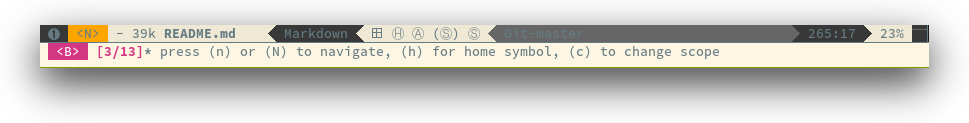
\includegraphics[width=.9\linewidth]{img/spacemacs-ahs-transient-state.png}
\end{center}
\hyperref[sec:orgae9b8c9]{Text scale transient state}:

\begin{center}
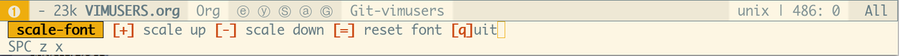
\includegraphics[width=.9\linewidth]{img/spacemacs-scale-transient-state.png}
\end{center}

\section{Differences between Vim, Evil and Spacemacs}
\label{sec:org60d05fe}
\begin{itemize}
\item The \texttt{​,​} key does "repeat last \texttt{f}, \texttt{t}, \texttt{F}, or \texttt{T} command in
opposite direction in \texttt{Vim}, but in Spacemacs it is the major mode specific
leader key by default (which can be set on another key binding in the
dotfile).
\end{itemize}

Send a PR to add the differences you found in this section.

\subsection{The vim-surround case}
\label{sec:orgb0b6265}
There is one obvious visible difference though. It is not between \texttt{Evil} and
\texttt{Vim} but between Spacemacs and \href{https://github.com/tpope/vim-surround}{vim-surround}: in visual mode the \texttt{surround} command is on \texttt{S}
in \texttt{vim-surround} whereas it is on \texttt{s} in Spacemacs.

This is something that can surprise some Vim users so here are some motivations
behind this change:
\begin{itemize}
\item \texttt{s} and \texttt{c} do the same thing in \texttt{visual state},
\item \texttt{s} is only useful to delete \emph{one} character and add more than one character
which is a \emph{very} narrow use case
\item \texttt{c} accept motions and can do everything \texttt{s} can do in \texttt{normal state}
(note that this is also true for \texttt{r} but \texttt{r} is more useful because it
stays in \texttt{normal state})
\item \texttt{surround} command is just a more powerful command than \texttt{s}.
\end{itemize}

If you are not convinced, then here is the snippet to revert back to the default
\texttt{Vim + vim-surround} setup (add it to your \texttt{dotspacemacs/user-config} function or
your \texttt{\textasciitilde{}/.spacemacs}):

\begin{verbatim}
(evil-define-key 'visual evil-surround-mode-map "s" 'evil-substitute)
(evil-define-key 'visual evil-surround-mode-map "S" 'evil-surround-region)
\end{verbatim}

\section{Evil plugins}
\label{sec:org367bb0f}
Spacemacs ships with the following evil plugins:

\begin{center}
\begin{tabular}{ll}
Mode & Description\\
\hline
\href{https://github.com/wcsmith/evil-args}{evil-args} & motions and text objects for arguments\\
\href{https://github.com/Dewdrops/evil-exchange}{evil-exchange} & port of \href{https://github.com/tommcdo/vim-exchange}{vim-exchange}\\
\href{https://github.com/cofi/evil-indent-textobject}{evil-indent-textobject} & add text object based on indentation level\\
\href{https://github.com/redguardtoo/evil-matchit}{evil-matchit} & port of \href{http://www.vim.org/scripts/script.php?script\_id=39}{matchit.vim}\\
\href{https://github.com/redguardtoo/evil-nerd-commenter}{evil-nerd-commenter} & port of \href{https://github.com/scrooloose/nerdcommenter}{nerdcommenter}\\
\href{https://github.com/cofi/evil-numbers}{evil-numbers} & like \texttt{C-a} and \texttt{C-x} in vim\\
\href{https://github.com/juanjux/evil-search-highlight-persist}{evil-search-highlight-persist} & emulation of hlsearch behavior\\
\href{https://github.com/timcharper/evil-surround}{evil-surround} & port of \href{https://github.com/tpope/vim-surround}{vim-surround}\\
\href{https://github.com/bling/evil-visualstar}{evil-visualstar} & search for current selection with \texttt{*}\\
\href{https://github.com/jaypei/emacs-neotree}{NeoTree} & mimic \href{https://github.com/scrooloose/nerdtree}{NERD Tree}\\
\end{tabular}
\end{center}

\section{Binding keys}
\label{sec:org61d8d49}
Key sequences are bound to commands in Emacs in various keymaps. The most basic
map is the \texttt{global-map}. Setting a key binding in the \texttt{global-map} is achieved
with the function \texttt{global-set-key}. Example to bind a key to the command
\texttt{forward-char}:

\begin{verbatim}
(global-set-key (kbd "C-]") 'forward-char)
\end{verbatim}

The \texttt{kbd} macro accepts a string describing a key sequence. The \texttt{global-map} is
often shadowed by other maps. For example, \texttt{evil-mode} defines keymaps that
target states (or modes in vim terminology). Here is an example that creates the
same binding as above but only in \texttt{insert state} (\texttt{define-key} is a built-in
function. \texttt{Evil-mode} has its own functions for defining keys).

\begin{verbatim}
(define-key evil-insert-state-map (kbd "C-]") 'forward-char)
\end{verbatim}

Perhaps most importantly for Spacemacs is the use of the bind-map package to
bind keys behind a leader key.
This is where most of the Spacemacs bindings live. Binding keys behind the
leader key is achieved with the functions \texttt{spacemacs/set-leader-keys} and
\texttt{spacemacs/set-leader-keys-for-major-mode}, example:

\begin{verbatim}
(spacemacs/set-leader-keys "C-]" 'forward-char)
(spacemacs/set-leader-keys-for-major-mode 'emacs-lisp-mode "C-]" 'forward-char)
\end{verbatim}

These functions use a macro like \texttt{kbd} to translate the key sequences for you.
The second function, \texttt{spacemacs/set-leader-keys-for-major-mode}, binds the key
only in the specified mode. The second key binding is active only when the
major mode is \texttt{emacs-lisp}.

Finally, one should be aware of prefix keys. Essentially, all keymaps can be
nested. Nested keymaps are used extensively in spacemacs, and in vanilla Emacs
for that matter. For example, \texttt{SPC a} points to key bindings for "applications",
like \texttt{SPC a c} for \texttt{calc-dispatch}. Nesting bindings is easy.

\begin{verbatim}
(spacemacs/declare-prefix "]" "bracket-prefix")
(spacemacs/set-leader-keys "]]" 'double-bracket-command)
\end{verbatim}

The first line declares \texttt{SPC ]} to be a prefix and the second binds the key
sequence \texttt{SPC ]]} to the corresponding command. The first line is actually
unnecessary to create the prefix, but it will give your new prefix a name that
key-discovery tools can use (e.g., which-key).

There is much more to say about bindings keys, but these are the basics. Keys
can be bound in your \texttt{\textasciitilde{}/.spacemacs} file or in individual layers.

\section{GUI Elements}
\label{sec:org54f4a14}
Spacemacs has a minimalistic and distraction free graphical UI:
\begin{itemize}
\item custom \href{https://github.com/milkypostman/powerline}{powerline} mode-line \hyperref[sec:org5995c01]{with color feedback} according to current \href{https://github.com/flycheck/flycheck}{Flycheck} status
\item Unicode symbols for minor mode lighters which appear in the mode-line
\item \hyperref[sec:org91d20ad]{custom fringe bitmaps} and error feedbacks for \href{https://github.com/flycheck/flycheck}{Flycheck}
\end{itemize}

\subsection{Color themes}
\label{sec:org18d2521}
The official Spacemacs theme is \href{https://github.com/nashamri/spacemacs-theme}{spacemacs-dark} and it is the default theme
installed when you first started Spacemacs. There are two variants of the
theme, a dark one and a light one. Some aspects of these themes can be customized
in the function \texttt{dotspacemacs/user-init} of your \texttt{\textasciitilde{}/.spacemacs}:
\begin{itemize}
\item the comment background with the boolean \texttt{spacemacs-theme-comment-bg}
\item the height of org section titles with \texttt{spacemacs-theme-org-height}
\end{itemize}

It is possible to define your default themes in your \texttt{\textasciitilde{}/.spacemacs} with the
variable \texttt{dotspacemacs-themes}. For instance, to specify \texttt{spacemacs-light},
\texttt{leuven} and \texttt{zenburn}:

\begin{verbatim}
(setq-default dotspacemacs-themes '(spacemacs-light leuven zenburn))
\end{verbatim}

\begin{center}
\begin{tabular}{ll}
Key Binding & Description\\
\hline
\texttt{SPC T n} & switch to next theme listed in \texttt{dotspacemacs-themes}.\\
\texttt{SPC T s} & select a theme using a \texttt{helm} buffer.\\
\end{tabular}
\end{center}

You can see samples of all included themes in this \href{http://themegallery.robdor.com}{theme gallery} from \href{http://www.twitter.com/robmerrell}{Rob Merrell}.

\textbf{Note}:
\begin{itemize}
\item You don't need to explicitly list in a layer the theme packages you are
defining in \texttt{dotspacemacs-themes}, Spacemacs is smart enough to remove those
packages from the list of orphans.
\item Due to the inner working of themes in Emacs, switching theme during the same
session may have some weird side effects. Although these side effects should
be pretty rare.
\item In the terminal version of Emacs, color themes will not render correctly as
colors are rendered by the terminal and not by emacs. You will probably have
to change your terminal color palette. More explanations can be found on
\href{https://github.com/sellout/emacs-color-theme-solarized\#important-note-for-terminal-users}{emacs-color-theme-solarized webpage}.
\end{itemize}

\textbf{Hint}: If you are an \texttt{Org} user, \href{https://github.com/fniessen/emacs-leuven-theme}{leuven-theme} is amazing ;-)

\subsection{Font}
\label{sec:org392fef9}
The default font used by Spacemacs is \href{https://github.com/adobe-fonts/source-code-pro}{Source Code Pro} by Adobe. It is
recommended to install it on your system if you wish to use it.

To change the default font set the variable \texttt{dotspacemacs-default-font} in your
\texttt{.spacemacs} file. By default its value is:

\begin{verbatim}
(setq-default dotspacemacs-default-font '("Source Code Pro"
                                          :size 13
                                          :weight normal
                                          :width normal
                                          :powerline-scale 1.1))
\end{verbatim}

If the specified font is not found, the fallback one will be used (depends on
your system). Also note that changing this value has no effect if you are
running Emacs in terminal.

The properties should be pretty straightforward, it is possible to set any valid
property of a \href{http://www.gnu.org/software/emacs/manual/html\_node/elisp/Low\_002dLevel-Font.html}{font-spec}:
\begin{itemize}
\item \texttt{:family} Font family or fontset (a string).
\item \texttt{:width} Relative character width. This should be one of the symbols:
\begin{itemize}
\item ultra-condensed
\item extra-condensed
\item condensed
\item semi-condensed
\item normal
\item semi-expanded
\item expanded
\item extra-expanded
\item ultra-expanded
\end{itemize}
\item \texttt{:height} The height of the font. In the simplest case, this is an integer
in units of 1/10 point.
\item \texttt{:weight} Font weight- one of the symbols (from densest to faintest):
\begin{itemize}
\item ultra-bold
\item extra-bold
\item bold
\item semi-bold
\item normal
\item semi-light
\item light
\item extra-light
\item ultra-light
\end{itemize}
\item \texttt{:slant} Font slant- one of the symbols:
\begin{itemize}
\item italic
\item oblique
\item normal
\item reverse-italic
\item reverse-oblique
\end{itemize}
\item \texttt{:size} The font size- either a non-negative integer that specifies the
pixel size, or a floating-point number that specifies the point size.
\item \texttt{:adstyle} Additional typographic style information for the font, such as
'sans'. The value should be a string or a symbol.
\item \texttt{:registry} The charset registry and encoding of the font, such as
'iso8859-1'. The value should be a string or a symbol.
\item \texttt{:script} The script that the font must support (a symbol).
\end{itemize}

The special property \texttt{:powerline-scale} is Spacemacs specific and it is for
quick tweaking of the mode-line height in order to avoid crappy rendering of the
separators like on the following screenshot (default value is 1.1).

\begin{center}

\includegraphics[width=.9\linewidth]{img/crappy-powerline-separators.png}
\end{center}
\emph{Ugly separators}

\subsection{GUI Toggles}
\label{sec:orgc68c68f}
Some graphical UI indicators can be toggled on and off (toggles start with \texttt{t}
and \texttt{T}):

\begin{center}
\begin{tabular}{ll}
Key Binding & Description\\
\hline
\texttt{SPC t 8} & highlight any character past the 80th column\\
\texttt{SPC t f} & display the fill column (by default the fill column is set to 80)\\
\texttt{SPC t h h} & toggle highlight of the current line\\
\texttt{SPC t h i} & toggle highlight indentation levels\\
\texttt{SPC t h c} & toggle highlight indentation current column\\
\texttt{SPC t h s} & toggle syntax highlighting\\
\texttt{SPC t i} & toggle indentation guide at point\\
\texttt{SPC t l} & toggle truncate lines\\
\texttt{SPC t L} & toggle visual lines\\
\texttt{SPC t n} & toggle line numbers\\
\texttt{SPC t v} & toggle smooth scrolling\\
\end{tabular}
\end{center}

\begin{center}
\begin{tabular}{ll}
Key Binding & Description\\
\hline
\texttt{SPC T \textasciitilde{}} & display \texttt{\textasciitilde{}} in the fringe on empty lines\\
\texttt{SPC T F} & toggle frame fullscreen\\
\texttt{SPC T f} & toggle display of the fringe\\
\texttt{SPC T m} & toggle menu bar\\
\texttt{SPC T M} & toggle frame maximize\\
\texttt{SPC T t} & toggle tool bar\\
\texttt{SPC T T} & toggle frame transparency and enter transparency transient state\\
\end{tabular}
\end{center}

\textbf{Note}: These toggles are all available via the \texttt{helm-spacemacs-help} interface
(press \texttt{SPC h SPC} to display the \texttt{helm-spacemacs-help} buffer).

\begin{enumerate}
\item Global line numbers
\label{sec:orgc5a5a1b}
Line numbers can be toggled on in all \texttt{prog-mode} and \texttt{text-mode} buffers by
setting the \texttt{dotspacemacs-line-numbers} variable in your \texttt{\textasciitilde{}/.spacemacs} to \texttt{t}.

\begin{verbatim}
(setq-default dotspacemacs-line-numbers t)
\end{verbatim}

If it is set to \texttt{relative}, line numbers are show in a relative way:

\begin{verbatim}
(setq-default dotspacemacs-line-numbers 'relative)
\end{verbatim}

\texttt{dotspacemacs-line-numbers} can also be set to a property list for finer control
over line numbers activation.

Available properties:

\begin{center}
\begin{tabular}{ll}
Property & Description\\
\hline
\texttt{:disabled-for-modes} & list of major modes where line numbering is inhibited\\
\texttt{:enabled-for-modes} & disable for all major modes except those listed. Takes precedence over \texttt{:disabled-for-modes}\\
\texttt{:relative} & if non-nil, line numbers are relative to the position of the cursor\\
\texttt{:size-limit-kb} & size limit in kilobytes after which line numbers are not activated\\
\end{tabular}
\end{center}

Examples:

Disable line numbers in dired-mode, doc-view-mode, markdown-mode, org-mode,
pdf-view-mode, text-mode as well as buffers over 1Mb:

\begin{verbatim}
(setq-default dotspacemacs-lines-numbers '(:relative nil
                                           :disabled-for-modes dired-mode
                                                               doc-view-mode
                                                               markdown-mode
                                                               org-mode
                                                               pdf-view-mode
                                                               text-mode
                                           :size-limit-kb 1000))
\end{verbatim}

Relative line numbers only in c-mode and c++ mode with a size limit of \texttt{dotspacemacs-large-file-size}:

\begin{verbatim}
(setq-default dotspacemacs-lines-numbers '(:relative t
                                           :enabled-for-modes c-mode
                                                              c++-mode
                                           :size-limit-kb (* dotspacemacs-large-file-size 1000))
\end{verbatim}

Enable line numbers everywhere, except for buffers over 1Mb:

\begin{verbatim}
(setq-default dotspacemacs-lines-numbers '(:relative nil
                                           :size-limit-kb 1000))
\end{verbatim}

Enable line numbers only in programming modes, except for c-mode and c++ mode:

\begin{verbatim}
(setq-default dotspacemacs-lines-numbers '(:relative nil
                                           :enabled-for-modes prog-mode
                                           :disabled-for-modes c-mode c++-mode
                                           :size-limit-kb (* dotspacemacs-large-file-size 1000))
\end{verbatim}
\end{enumerate}

\subsection{Mode-line}
\label{sec:org2649cda}
The mode line is a heavily customized \href{https://github.com/milkypostman/powerline}{powerline} with the following capabilities:
\begin{itemize}
\item show the window number
\item color code for current state
\item show the number of search occurrences via anzu
\item toggle flycheck info
\item toggle battery info
\item toggle minor mode lighters
\end{itemize}

Reminder of the color codes for the states:

\begin{center}
\begin{tabular}{ll}
Evil State & Color\\
\hline
Normal & Orange\\
Insert & Green\\
Visual & Grey\\
Emacs & Blue\\
Motion & Purple\\
Replace & Chocolate\\
Lisp & Pink\\
Iedit/Iedit-Insert & Red\\
\end{tabular}
\end{center}

Some elements can be dynamically toggled:

\begin{center}
\begin{tabular}{ll}
Key Binding & Description\\
\hline
\texttt{SPC t m b} & toggle the battery status\\
\texttt{SPC t m c} & toggle the \texttt{org} task clock (available in \texttt{org} layer)\\
\texttt{SPC t m m} & toggle the minor mode lighters\\
\texttt{SPC t m M} & toggle the major mode\\
\texttt{SPC t m n} & toggle the cat! (if \texttt{colors} layer is declared in your dotfile)\\
\texttt{SPC t m p} & toggle the point character position\\
\texttt{SPC t m t} & toggle the time\\
\texttt{SPC t m T} & toggle the mode line itself\\
\texttt{SPC t m v} & toggle the version control info\\
\texttt{SPC t m V} & toggle the new version lighter\\
\end{tabular}
\end{center}

\begin{enumerate}
\item Powerline font installation for terminal-mode users
\label{sec:org545e9af}
Users who run Emacs in terminal mode may need to install the \href{https://github.com/powerline/fonts}{Powerline patched
fonts} and configure their terminal clients to use them to make the Powerline
separators render correctly.

\item Flycheck integration
\label{sec:org5995c01}
When \href{https://github.com/flycheck/flycheck}{Flycheck} minor mode is enabled, a new element appears showing the number of
errors, warnings and info.

\begin{center}

\includegraphics[width=.9\linewidth]{img/powerline-wave.png}
\end{center}
\emph{Flycheck integration in mode-line}

\item Anzu integration
\label{sec:org1efff25}
\href{https://github.com/syohex/emacs-anzu}{Anzu} shows the number of occurrence when performing a search. Spacemacs
integrates nicely the Anzu status by displaying it temporarily when \texttt{n} or \texttt{N}
are being pressed. See the \texttt{5/6} segment on the screenshot below.

\begin{center}

\includegraphics[width=.9\linewidth]{img/powerline-anzu.png}
\end{center}
\emph{Anzu integration in mode-line}

\item Battery status integration
\label{sec:org94ffc5e}
\href{https://github.com/lunaryorn/fancy-battery.el}{fancy-battery} displays the percentage of total charge of the battery as well as
the time remaining to charge or discharge completely the battery.

A color code is used for the battery status:

\begin{center}
\begin{tabular}{ll}
Battery State & Color\\
\hline
Charging & Green\\
Discharging & Orange\\
Critical & Red\\
\end{tabular}
\end{center}

Note the these colors may vary depending on your theme.

\item Powerline separators
\label{sec:org85ed33b}
It is possible to easily customize the \texttt{powerline separator} by setting the
\texttt{powerline-default-separator} variable in your \texttt{\textasciitilde{}./spacemacs} and then
recompiling the modeline. For instance if you want to set back the separator to
the well-known \texttt{arrow} separator add the following snippet to your configuration
file:

\begin{verbatim}
(defun dotspacemacs/user-config ()
  "This is were you can ultimately override default Spacemacs configuration.
This function is called at the very end of Spacemacs initialization."
  (setq powerline-default-separator 'arrow))
\end{verbatim}

To save you the time to try all the possible separators provided by the
powerline, here is an exhaustive set of screenshots:

\begin{center}
\begin{tabular}{ll}
Separator & Screenshot\\
\hline
\texttt{alternate} & \begin{center}

\includegraphics[width=.9\linewidth]{img/powerline-alternate.png}
\end{center}\\
\texttt{arrow} & \begin{center}

\includegraphics[width=.9\linewidth]{img/powerline-arrow.png}
\end{center}\\
\texttt{arrow-fade} & \begin{center}

\includegraphics[width=.9\linewidth]{img/powerline-arrow-fade.png}
\end{center}\\
\texttt{bar} & \begin{center}

\includegraphics[width=.9\linewidth]{img/powerline-bar.png}
\end{center}\\
\texttt{box} & \begin{center}

\includegraphics[width=.9\linewidth]{img/powerline-box.png}
\end{center}\\
\texttt{brace} & \begin{center}

\includegraphics[width=.9\linewidth]{img/powerline-brace.png}
\end{center}\\
\texttt{butt} & \begin{center}

\includegraphics[width=.9\linewidth]{img/powerline-butt.png}
\end{center}\\
\texttt{chamfer} & \begin{center}

\includegraphics[width=.9\linewidth]{img/powerline-chamfer.png}
\end{center}\\
\texttt{contour} & \begin{center}

\includegraphics[width=.9\linewidth]{img/powerline-contour.png}
\end{center}\\
\texttt{curve} & \begin{center}

\includegraphics[width=.9\linewidth]{img/powerline-curve.png}
\end{center}\\
\texttt{rounded} & \begin{center}

\includegraphics[width=.9\linewidth]{img/powerline-rounded.png}
\end{center}\\
\texttt{roundstub} & \begin{center}

\includegraphics[width=.9\linewidth]{img/powerline-roundstub.png}
\end{center}\\
\texttt{slant} & \begin{center}

\includegraphics[width=.9\linewidth]{img/powerline-slant.png}
\end{center}\\
\texttt{wave} & \begin{center}

\includegraphics[width=.9\linewidth]{img/powerline-wave.png}
\end{center}\\
\texttt{zigzag} & \begin{center}

\includegraphics[width=.9\linewidth]{img/powerline-zigzag.png}
\end{center}\\
\texttt{nil} & \begin{center}

\includegraphics[width=.9\linewidth]{img/powerline-nil.png}
\end{center}\\
\end{tabular}
\end{center}

\item Minor Modes
\label{sec:orga4f3aaa}
Spacemacs uses \href{http://www.emacswiki.org/emacs/DiminishedModes}{diminish} mode to reduce the size of minor mode indicators:

The minor mode area can be toggled on and off with \texttt{SPC t m m}

Unicode symbols are displayed by default. Setting the variable
\texttt{dotspacemacs-mode-line-unicode-symbols} to \texttt{nil} in your \texttt{\textasciitilde{}/.spacemacs} will
display ASCII characters instead (may be useful in terminal if you cannot set an
appropriate font).

The letters displayed in the mode-line correspond to the key bindings used to
toggle them.

Some toggle have two flavors: local and global. The global version of the toggle
can be reached using the \texttt{control} key.

\begin{center}
\begin{tabular}{llll}
Key Binding & Unicode & ASCII & Mode\\
\hline
\texttt{SPC t -} & \texttt{⊝} & - & \href{http://emacswiki.org/emacs/centered-cursor-mode.el}{centered-cursor}  mode\\
\texttt{SPC t 8} & \texttt{⑧} & 8 & toggle highlight of characters for long lines\\
\texttt{SPC t C-8} & \texttt{⑧} & 8 & global toggle highlight of characters for long lines\\
\texttt{SPC t C-{}-} & \texttt{⊝} & - & global centered cursor\\
\texttt{SPC t a} & \texttt{ⓐ} & a & auto-completion\\
\texttt{SPC t c} & \texttt{ⓒ} & c & camel case motion with subword mode\\
\texttt{none} & \texttt{ⓔ} & e & \href{https://github.com/edwtjo/evil-org-mode}{evil-org} mode\\
\texttt{SPC t E e} & \texttt{Ⓔe} & Ee & emacs editing style (holy mode)\\
\texttt{SPC t E h} & \texttt{Ⓔh} & Eh & hybrid editing style (hybrid mode)\\
\texttt{SPC t f} & \texttt{ⓕ} & f & fill-column-indicator mode\\
\texttt{SPC t F} & \texttt{Ⓕ} & F & auto-fill mode\\
\texttt{SPC t g} & \texttt{ⓖ} & g & \href{https://github.com/roman/golden-ratio.el}{golden-ratio} mode\\
\texttt{SPC t h i} & \texttt{ⓗi} & hi & toggle highlight indentation levels\\
\texttt{SPC t h c} & \texttt{ⓗc} & hc & toggle highlight indentation current column\\
\texttt{SPC t i} & \texttt{ⓘ} & i & indentation guide\\
\texttt{SPC t C-i} & \texttt{ⓘ} & i & global indentation guide\\
\texttt{SPC t I} & \texttt{Ⓘ} & I & aggressive indent mode\\
\texttt{SPC t K} & \texttt{Ⓚ} & K & which-key mode\\
\texttt{SPC t p} & \texttt{ⓟ} & p & \href{https://github.com/Fuco1/smartparens}{smartparens} mode\\
\texttt{SPC t C-p} & \texttt{ⓟ} & p & global smartparens\\
\texttt{SPC t s} & \texttt{ⓢ} & s & syntax checking (flycheck)\\
\texttt{SPC t S} & \texttt{Ⓢ} & S & enabled in \href{../layers/+checkers/spell-checking/README.org}{spell checking layer} (flyspell)\\
\texttt{SPC t w} & \texttt{ⓦ} & w & whitespace mode\\
\texttt{SPC t C-w} & \texttt{ⓦ} & w & global whitespace\\
\texttt{SPC t W} & \texttt{Ⓦ} & W & automatic whitespace cleanup (see \texttt{dotspacemacs-whitespace-cleanup})\\
\texttt{SPC t C-W} & \texttt{Ⓦ} & W & automatic whitespace cleanup globally\\
\texttt{SPC t y} & \texttt{ⓨ} & y & \href{https://github.com/capitaomorte/yasnippet}{yasnippet} mode\\
\end{tabular}
\end{center}

\item Customizing the mode-line
\label{sec:org294bff0}
Spacemacs uses \href{https://github.com/TheBB/spaceline}{Spaceline} to provide its mode-line. It consists of a number of
\emph{segments} arranged on the left and right sides. These are defined in the
variables \texttt{spaceline-left} and \texttt{spaceline-right}. Segments can be defined using
\texttt{spaceline-define-segment}, and added to the appropriate location in the left or
right hand side variables.

Please see the Spaceline documentation for more information.
\end{enumerate}

\section{Layouts and workspaces}
\label{sec:org5de7fb6}
Layouts are window configurations with buffer isolation, each layout can define
several workspaces (think of them as sub-layouts) sharing the same list of
buffers as their parent layout.

\subsection{Layouts}
\label{sec:orgdb625b5}
A layout is a window configuration associated with a list of buffers. The list
of buffers can be an arbitrarily chosen set of buffers. Spacemacs provides
some facilities to create meaningful sets of buffers, for instance the buffers
related to a projectile project.

The name of the current layout appears in the mode-line at the far left (first
element of the mode-line).

To create a new layout type a layout number that does not exist yet.
For instance if you have two layouts currently then type \texttt{SPC l 3} to create a
third layout.

\subsubsection{The default layout}
\label{sec:org31b22dd}
The \texttt{default} layout (the layout created at the startup of Emacs) is not
displayed in the mode-line but it is possible to display it by setting the
variable \texttt{dotspacemacs-display-default-layout} to \texttt{t}.

Its name is "default" by default but it can be changed by setting the variable
\texttt{dotspacemacs-default-layout-name}.

The \texttt{default} layout is special because it has a global scope which means that
all the opened buffers belong to it. So using only the \texttt{default} layout feels
like not using layouts at all.

\subsubsection{Project layouts}
\label{sec:org8d5ce86}
A project layout is bound to a projectile project. To create a project layout
use \texttt{SPC p l}.

The name of the layout is the name of the project root directory.

\subsubsection{Custom Layouts}
\label{sec:org5768222}
Custom layouts can be defined using the macro \texttt{spacemacs|define-custom-layout},
they are accessible via \texttt{SPC l o}.

By convention the name of a custom layout should start with \texttt{@}.

Example of custom layout definition for \texttt{ERC} buffers:

\begin{verbatim}
(spacemacs|define-custom-layout "@ERC"
  :binding "E"
  :body
  (progn
    ;; hook to add all ERC buffers to the layout
    (defun spacemacs-layouts/add-erc-buffer-to-persp ()
      (persp-add-buffer (current-buffer)
                        (persp-get-by-name
                         erc-spacemacs-layout-name)))
    (add-hook 'erc-mode-hook #'spacemacs-layouts/add-erc-buffer-to-persp)
    ;; Start ERC
    (call-interactively 'erc)))
\end{verbatim}

Then use \texttt{SPC l o E} to start ERC inside its own layout. Any new ERC buffer
will be part of the custom layout.

Some custom layouts that ship with Spacemacs:

\begin{center}
\begin{tabular}{lll}
Name & Key Binding & Description\\
\hline
@Spacemacs & \texttt{e} & Custom perspective containing all buffers of \texttt{\textasciitilde{}/.emacs.d}\\
@ERC & \texttt{E} & Custom perspective containing all ERC buffers (needs the erc layer enabled)\\
@RCIRC & \texttt{i} & Custom perspective containing all RCIRC buffers (needs the rcirc layer enabled)\\
@Org & \texttt{o} & Custom perspective containing all the \texttt{org-agenda} buffers\\
\end{tabular}
\end{center}

\subsubsection{Save/Load layouts into a file}
\label{sec:org00d18e3}
With \texttt{SPC l s} and \texttt{SPC l L} you can save and load layouts to/from a file.

\textbf{Note:} By default, Spacemacs will automatically save the layouts under the name
\texttt{persp-auto-save}.

Setting the variable \texttt{dotspacemacs-auto-resume-layouts} to \texttt{t} will
automatically resume the last saved layouts.

\subsubsection{Layout key bindings}
\label{sec:org450e0bb}
The key bindings are registered in a transient state. The docstring of the
transient state displays the existing layouts and the currently active
layout has square brackets. Pressing a layout number will activate it (or
create a new one) and exit the transient state. It is possible to just preview a
layout with \texttt{Ctrl-<number>}. Pressing \texttt{TAB} will activate the previously
selected layout.

Press \texttt{?} to toggle the full help.

\begin{center}
\begin{tabular}{ll}
Key Binding & Description\\
\hline
\texttt{SPC l} & activate the transient- state\\
\texttt{?} & toggle the documentation\\
\texttt{[0..9]} & switch to nth layout\\
\texttt{[C-0..C-9]} & switch to nth layout and keep the transient state active\\
\texttt{<tab>} & switch to the latest layout\\
\texttt{a} & add a buffer to the current layout\\
\texttt{A} & add all the buffers from another layout in the current one\\
\texttt{b} & select a buffer in the current layout\\
\texttt{d} & delete the current layout and keep its buffers\\
\texttt{D} & delete the other layouts and keep their buffers\\
\texttt{h} & go to default layout\\
\texttt{C-h} & previous layout in list\\
\texttt{l} & select/create a layout with helm\\
\texttt{L} & load layouts from file\\
\texttt{C-l} & next layout in list\\
\texttt{n} & next layout in list\\
\texttt{N} & previous layout in list\\
\texttt{o} & open a custom layout\\
\texttt{p} & previous layout in list\\
\texttt{r} & remove current buffer from layout\\
\texttt{R} & rename current layout\\
\texttt{s} & save layouts\\
\texttt{t} & display a buffer without adding it to the current layout\\
\texttt{w} & workspaces transient state (needs eyebrowse layer enabled)\\
\texttt{x} & kill current layout with its buffers\\
\texttt{X} & kill other layouts with their buffers\\
\end{tabular}
\end{center}

\subsection{Workspaces}
\label{sec:org94e6d64}
Workspaces are sub-layouts, they allow to define multiple layouts into a given
layout, those layouts share the same buffer as the parent layout.

The currently active workspace number is displayed before the window number,
for instance "➊|➍" or "1|4" means the fourth window of the first workspace.

Any new layout comes with a default workspace which is the workspace 1.

Switching to a workspace that does not exist in the current layout will create a
new one. For instance at startup you can press \texttt{SPC l w 2} to create the
workspace 2 in the \texttt{default} layout.

When created a workspace is anonymous, you can give them a name with
\texttt{SPC l w R}.

\subsubsection{Workspace key bindings}
\label{sec:org9e65e87}
The key bindings are registered in a transient state. The docstring of the
transient state displays the existing workspaces and the currently active
workspace has square brackets. Pressing a workspace number will activate it (or
create a new one) and exit the transient state. It is possible to just preview a
workspace with \texttt{Ctrl-<number>}. Pressing \texttt{TAB} will activate the previously
selected workspace.

Press \texttt{?} to toggle the full help.

\begin{center}
\begin{tabular}{ll}
Key Binding & Description\\
\hline
\texttt{SPC l w} & activate the transient state\\
\texttt{?} & toggle the documentation\\
\texttt{[0..9]} & switch to nth workspace\\
\texttt{[C-0..C-9]} & switch to nth workspace and keep the transient state active\\
\texttt{TAB} & switch to last active workspace\\
\texttt{d} & close current workspace\\
\texttt{n} or \texttt{l} & switch to next workspace\\
\texttt{N} or \texttt{p} or \texttt{h} & switch to previous workspace\\
\texttt{R} & set a tag to the current workspace\\
\texttt{w} & switched to tagged workspace\\
\end{tabular}
\end{center}

There are also some handy globally available key bindings related to workspaces:

\begin{center}
\begin{tabular}{ll}
Key Binding & Description\\
\hline
\texttt{gt} & go to next workspace\\
\texttt{gT} & go to previous workspace\\
\texttt{SPC b W} & go to workspace and window by buffer\\
\end{tabular}
\end{center}

\section{Commands}
\label{sec:org06a7411}
\subsection{Vim key bindings}
\label{sec:orgaf2e59f}
Spacemacs is based on \texttt{Vim} modal user interface to navigate and edit text. If
you are not familiar with the \texttt{Vim} way of editing text you can try the
\href{https://github.com/syl20bnr/evil-tutor}{evil-tutor} lessons by pressing \texttt{SPC h T} at any time.

\subsubsection{Escaping}
\label{sec:org0322b3d}
Spacemacs uses \href{https://github.com/syl20bnr/evil-escape}{evil-escape} to
easily switch between \texttt{insert state} and \texttt{normal state} by quickly pressing the
\texttt{fd} keys.

The choice of \texttt{fd} was made to be able to use the same sequence to escape from
"everything" in Emacs:
\begin{itemize}
\item escape from all stock evil states to normal state
\item escape from evil-lisp-state to normal state
\item escape from evil-iedit-state to normal state
\item abort evil ex command
\item quit minibuffer
\item abort isearch
\item quit magit buffers
\item quit help buffers
\item quit apropos buffers
\item quit ert buffers
\item quit undo-tree buffer
\item quit paradox
\item quit gist-list menu
\item quit helm-ag-edit
\item hide neotree buffer
\end{itemize}

If you find yourself in a buffer where the Spacemacs (\texttt{SPC}) or Vim keybindings
don't work you can use this to get back to \texttt{normal state} (for example in \texttt{SPC
SPC customize} press \texttt{fd} to make \texttt{SPC b b} work again).

This sequence can be customized in your \texttt{\textasciitilde{}/.spacemacs}.
Example to set it to \texttt{jj}:

\begin{verbatim}
(defun dotspacemacs/user-config ()
  (setq-default evil-escape-key-sequence "jj"))
\end{verbatim}

\textbf{Note}: Although \texttt{jj} or \texttt{jk} are popular choices of vim users, these key
sequences are not optimal for Spacemacs. Indeed it is very easy in \texttt{visual
state} to press quickly \texttt{jj} and inadvertently escape to \texttt{normal state}.

\subsubsection{Executing Vim and Emacs ex/M-x commands}
\label{sec:orgf65b1d0}

\begin{center}
\begin{tabular}{ll}
Command & Key Binding\\
\hline
Vim (ex-command) & \texttt{:}\\
Emacs (M-x) & \texttt{SPC SPC}\\
\end{tabular}
\end{center}

The emacs command key \texttt{SPC} (executed after the leader key) can be changed
with the variable \texttt{dotspacemacs-emacs-command-key} of your \texttt{\textasciitilde{}/.spacemacs}.

\subsubsection{Leader key}
\label{sec:org2cdbc68}
On top of \texttt{Vim} modes (modes are called states in Spacemacs) there is a
special key called the leader key which once pressed gives a whole new keyboard
layer. The leader key is by default \texttt{SPC} (space). It is possible to change this
key with the variable \texttt{dotspacemacs-leader-key}.

\subsubsection{Additional text objects}
\label{sec:orgdc620fc}
Additional text objects are defined in Spacemacs:

\begin{center}
\begin{tabular}{ll}
Object & Description\\
\hline
\texttt{a} & an argument\\
\texttt{g} & the entire buffer\\
\texttt{\$} & text between \texttt{\$}\\
\texttt{*} & text between \texttt{*}\\
\texttt{8} & text between \texttt{/*} and \texttt{*/}\\
\texttt{\%} & text between \texttt{\%}\\
\texttt{\textbackslash{}vert} & text between \texttt{\textbackslash{}vert}\\
\end{tabular}
\end{center}

\subsection{Reserved prefix command for user}
\label{sec:org2c8c648}
\texttt{SPC o} and \texttt{SPC m o} are reserved for the user. Setting key bindings behind
these is \textbf{guaranteed} to never conflict with Spacemacs default key bindings.

\textbf{Example:} Put \texttt{(spacemacs/set-leader-keys "oc" 'org-capture)} inside
\texttt{dotspacemacs/user-config} in your \texttt{\textasciitilde{}/.spacemacs} file, to be able to use \texttt{SPC o
c} to run org mode capture.

\subsection{Completion}
\label{sec:org5b75cfe}
Spacemacs is powered by one of two incremental completion and selection
narrowing frameworks: \href{https://github.com/emacs-helm/helm}{Helm} (default) or \href{https://github.com/abo-abo/swiper}{Ivy}. To use Ivy, add the \texttt{ivy} layer to
your list of enabled layers. If the \texttt{ivy} layer is not enabled, Helm will be
enabled automatically. (Please note that, as Helm is the more mature of the two,
some functions may be unavailable if you choose Ivy.)

These completion systems are the central control towers of Spacemacs, they are
used to manage buffers, projects, search results, configuration layers, toggles
and more\ldots{}

Mastering your choice of completion system will make you a Spacemacs power user.

\subsubsection{Helm}
\label{sec:orga940194}
Do not hesitate to read the \href{https://github.com/emacs-helm/helm/wiki}{Helm documentation wiki}.

\begin{enumerate}
\item C-z and Tab switch
\label{sec:org137cc1a}
The command bound to \texttt{C-z} is much more useful than the one bound to Tab, so it
makes sense to swap them. It's also recommended \href{http://tuhdo.github.io/helm-intro.html}{here}.

\item Helm focus
\label{sec:org52dfc68}
If you find yourself unable to return focus to Helm (after a careless
mouse-click for example), use \texttt{SPC w b} to return focus to the minibuffer.

\item Helm transient state
\label{sec:org70b4995}
Spacemacs defines a \hyperref[sec:orgb0bb9d9]{transient state} for \texttt{Helm} to make it work like \href{https://github.com/Shougo/unite.vim}{Vim's Unite}
plugin.

Initiate the transient state with \texttt{M-SPC} or \texttt{s-M-SPC} while in a \texttt{Helm} buffer.

\begin{center}
\begin{tabular}{ll}
Key Binding & Description\\
\hline
\texttt{M-SPC} or \texttt{s-M-SPC} & initiate the transient state\\
\texttt{q} & quit transient state\\
\texttt{TAB} & switch to actions page and leave the transient state\\
\texttt{1} & execute action 0\\
\texttt{2} & execute action 1\\
\texttt{3} & execute action 2\\
\texttt{4} & execute action 3\\
\texttt{5} & execute action 4\\
\texttt{6} & execute action 5\\
\texttt{7} & execute action 6\\
\texttt{8} & execute action 7\\
\texttt{9} & execute action 8\\
\texttt{0} & execute action 9\\
\texttt{a} & switch to actions page\\
\texttt{g} & go to first candidate\\
\texttt{G} & go to last candidate\\
\texttt{h} & go to previous source\\
\texttt{j} & select next candidate\\
\texttt{k} & select previous candidate\\
\texttt{l} & go to next source\\
\texttt{t} & mark current candidate\\
\texttt{T} & mark all candidates\\
\texttt{v} & execute persistent action\\
\end{tabular}
\end{center}
\end{enumerate}

\subsubsection{Ivy}
\label{sec:orgb30d5c4}
If you choose \texttt{ivy} as completion system, make sure to read \href{http://oremacs.com/swiper/}{official manual}. In
case you don't want to read everything, at least familiarise with \href{http://oremacs.com/swiper/\#minibuffer-key-bindings}{minibuffer key
bindings}. Some useful key bindings are presented in following table.

\begin{center}
\begin{tabular}{ll}
Key Binding & Description\\
\hline
\texttt{C-m} or \texttt{RET} & call default action on current candidate\\
\texttt{M-o} & show the list of valid actions on current candidate (then press any of described keys to execute it)\\
\texttt{C-M-m} & the same as \texttt{RET} but doesn't close completion minibuffer\\
\texttt{C-M-o} & the same as \texttt{M-o} but doesn't close completion minibuffer\\
\texttt{C-'} & use avy to quickly select completion on current page (sometimes faster than using arrows)\\
\end{tabular}
\end{center}

\subsection{Discovering}
\label{sec:orga987131}
\subsubsection{Key bindings}
\label{sec:org8f0b6fd}
\begin{enumerate}
\item Which-key
\label{sec:orga0c9a72}
A help buffer is displayed each time the \texttt{SPC} key is pressed in normal mode.
It lists the available key bindings and their associated commands.

By default the \href{https://github.com/justbur/emacs-which-key}{which-key} buffer will be displayed quickly after the key has been
pressed. You can change the delay by setting the variable
\texttt{dotspacemacs-which-key-delay} to your liking (the value is in second).

\item Helm describe key bindings
\label{sec:orgdd446a9}
It is possible to search for specific key bindings by pressing \texttt{SPC ?}.

To narrow the list to some key bindings using the leader key type a pattern like
this regular expression: \texttt{SPC\textbackslash{} b} which would list all \texttt{buffer} related
bindings.
\end{enumerate}

\subsubsection{Getting help}
\label{sec:org661b949}
\texttt{Describe functions} are powerful Emacs introspection commands to get
information about functions, variables, modes etc. These commands are bound
thusly:

\begin{center}
\begin{tabular}{ll}
Key Binding & Description\\
\hline
\texttt{SPC h d b} & describe bindings in a \texttt{helm} buffer\\
\texttt{SPC h d c} & describe current character under point\\
\texttt{SPC h d d} & describe current expression under point\\
\texttt{SPC h d f} & describe a function\\
\texttt{SPC h d F} & describe a face\\
\texttt{SPC h d k} & describe a key\\
\texttt{SPC h d K} & describe a keymap\\
\texttt{SPC h d l} & copy last pressed keys that you can paste in gitter chat\\
\texttt{SPC h d m} & describe current modes\\
\texttt{SPC h d p} & describe a package (Emacs built-in function)\\
\texttt{SPC h d P} & describe a package (Spacemacs layer information)\\
\texttt{SPC h d s} & copy system information that you can paste in gitter chat\\
\texttt{SPC h d t} & describe a theme\\
\texttt{SPC h d v} & describe a variable\\
\end{tabular}
\end{center}

Other help key bindings:

\begin{center}
\begin{tabular}{ll}
Key Binding & Description\\
\hline
\texttt{SPC h SPC} & discover Spacemacs documentation, layers and packages using \texttt{helm}\\
\texttt{SPC h i} & search in info pages with the symbol at point\\
\texttt{SPC h k} & show top-level bindings with \texttt{which-key}\\
\texttt{SPC h m} & search available man pages\\
\texttt{SPC h n} & browse emacs news\\
\end{tabular}
\end{center}

Navigation key bindings in \texttt{help-mode}:

\begin{center}
\begin{tabular}{ll}
Key Binding & Description\\
\hline
\texttt{g b} or \texttt{[} & go back (same as clicking on \texttt{[back]} button)\\
\texttt{g f} or \texttt{]} & go forward (same as clicking on \texttt{[forward]} button)\\
\texttt{g h} & go to help for symbol under point\\
\end{tabular}
\end{center}

Reporting an issue:

\begin{center}
\begin{tabular}{ll}
Key Binding & Description\\
\hline
\texttt{SPC h I} & Open Spacemacs GitHub issue page with pre-filled information\\
\texttt{SPC u SPC h I} & Open Spacemacs GitHub issue page with pre-filled information - include last pressed keys\\
\end{tabular}
\end{center}

\emph{Note:} If these two bindings are used with the \texttt{*Backtrace*} buffer open, the
backtrace is automatically included

\subsubsection{Available layers}
\label{sec:org350e07f}
All layers can be easily discovered via \texttt{helm-spacemacs-help} accessible with
\texttt{SPC h SPC}.

The following helm actions are available:
\begin{itemize}
\item default: open the layer \texttt{README.org}
\item 2nd: open the layer \texttt{packages.el}
\end{itemize}

\begin{enumerate}
\item Available packages in Spacemacs
\label{sec:orgc395d59}
\texttt{helm-spacemacs-help} also lists all the packages available in Spacemacs. The
entry format is \texttt{(layer) packages}. If you type \texttt{flycheck} you'll be able to see
all the layers where \texttt{flycheck} is used.

The following helm actions are available on packages:
\begin{itemize}
\item default: go the package init function
\end{itemize}

\item New packages from ELPA repositories
\label{sec:org0092d35}
\texttt{package-list-packages} is where you can browse for all available packages in the
different Elpa repositories. It is possible to upgrade packages from there but
it is not recommended, use the \texttt{[Update Packages]} link on the Spacemacs startup
page instead.

Spacemacs uses \href{https://github.com/Bruce-Connor/paradox}{Paradox} instead of \texttt{package-list-packages} to list available
ELPA packages. Paradox enhances the package list buffer with better feedbacks,
new filters and Github information like the number of stars. Optionally you can
also star packages directly in the buffer.

\textbf{Important Note 1}: Installing a new package from \texttt{Paradox} won't make it
persistent. To install a package persistently you have to add it explicitly to a
configuration layer.

\textbf{Important Note 2}: Don't \emph{update} your packages from \texttt{Paradox} or
\texttt{package-list-packages} because they don't support the rollback feature of
Spacemacs.

\begin{center}
\begin{tabular}{ll}
Key Binding & Description\\
\hline
\texttt{SPC a k} & launch \texttt{paradox}\\
\texttt{/} & evil-search\\
\texttt{f k} & filter by keywords\\
\texttt{f r} & filter by regexp\\
\texttt{f u} & display only installed package with updates available\\
\texttt{h} & go left\\
\texttt{H} & show help (not accurate)\\
\texttt{j} & go down\\
\texttt{k} & go up\\
\texttt{l} & go right\\
\texttt{L} & show last commits\\
\texttt{n} & next search occurrence\\
\texttt{N} & previous search occurrence\\
\texttt{o} & open package homepage\\
\texttt{r} & refresh\\
\texttt{S P} & sort by package name\\
\texttt{S S} & sort by status (installed, available, etc\ldots{})\\
\texttt{S *} & sort by Github stars\\
\texttt{v} & \texttt{visual state}\\
\texttt{V} & \texttt{visual-line state}\\
\texttt{x} & execute (action flags)\\
\end{tabular}
\end{center}
\end{enumerate}

\subsubsection{Toggles}
\label{sec:orgf3cdc9b}
\texttt{helm-spacemacs-help} is also a central place to discover the available toggles.
To display only the toggles source press \texttt{C-l} (or in \hyperref[sec:org70b4995]{Helm transient state} you can
press just \texttt{l}).

The following helm actions are available on packages:
\begin{itemize}
\item default: toggle on/off
\end{itemize}

\textbf{Tips} Use \texttt{SPC h l} to resume the last helm session. It is handy to quickly
toggle on and off a toggle.

\subsection{Navigating}
\label{sec:org5eac294}
\subsubsection{Point/Cursor}
\label{sec:orga8012d1}
Navigation is performed using the Vi key bindings \texttt{hjkl}.

\begin{center}
\begin{tabular}{ll}
Key Binding & Description\\
\hline
\texttt{h} & move cursor left\\
\texttt{j} & move cursor down\\
\texttt{k} & move cursor up\\
\texttt{l} & move cursor right\\
\texttt{H} & move cursor to the top of the screen\\
\texttt{L} & move cursor to the bottom of the screen\\
\texttt{SPC j 0} & go to the beginning of line (and set a mark at the previous location in the line)\\
\texttt{SPC j \$} & go to the end of line (and set a mark at the previous location in the line)\\
\texttt{SPC t -} & lock the cursor at the center of the screen\\
\end{tabular}
\end{center}

\begin{enumerate}
\item Smooth scrolling
\label{sec:org3ed9fd4}
\href{https://github.com/aspiers/smooth-scrolling}{smooth-scrolling} prevent the point to jump when it reaches the top or
bottom of the screen. It is enabled by default.

On Windows, you may want to disable it. To disable the smooth scrolling set the
\texttt{dotspacemacs-smooth-scrolling} variable in your \texttt{\textasciitilde{}/.spacemacs} to \texttt{nil}:

\begin{verbatim}
(setq-default dotspacemacs-smooth-scrolling nil)
\end{verbatim}

You can also toggle smooth scrolling with \texttt{SPC t v}.
\end{enumerate}

\subsubsection{Vim motions with avy}
\label{sec:org2b3dfe2}
Spacemacs uses the \texttt{evil} integration of \href{https://github.com/abo-abo/avy}{avy} which enables the
invocation of \texttt{avy} during motions.

For instance, it is useful for deleting a set of visual lines from the current line.
Try the following sequence in a buffer containing some text: \texttt{d SPC j l}, followed by
selecting an avy candidate.

\begin{center}
\begin{tabular}{ll}
Key Binding & Description\\
\hline
\texttt{SPC j b} & go back to the previous location (before the jump)\\
\texttt{SPC j j} & initiate avy jump char\\
\texttt{SPC j w} & initiate avy jump word\\
\texttt{SPC j l} & initiate avy jump line\\
\end{tabular}
\end{center}

\begin{enumerate}
\item ace-link mode
\label{sec:org4f1ffe0}
Similar to \texttt{avy}, \href{https://github.com/abo-abo/ace-link}{ace-link} allows one to jump to any link in
\texttt{help-mode} and \texttt{info-mode} with two key strokes.

\begin{center}
\begin{tabular}{ll}
Key Binding & Description\\
\hline
\texttt{o} & initiate ace link mode in \texttt{help-mode} and \texttt{info-mode}\\
\end{tabular}
\end{center}
\end{enumerate}

\subsubsection{Unimpaired bindings}
\label{sec:orgd9bdff6}
Spacemacs comes with a built-in port of \href{https://github.com/tpope/vim-unimpaired}{tpope's vim-unimpaired}.

This plugin provides several pairs of bracket maps using \texttt{[} to denote
previous, and \texttt{]} as next.

\begin{center}
\begin{tabular}{ll}
KeyBindings & Description\\
\hline
\texttt{[ SPC} & Insert space above\\
\texttt{] SPC} & Insert space below\\
\texttt{[ b} & Go to previous buffer\\
\texttt{] b} & Go to next buffer\\
\texttt{[ f} & Go to previous file in directory\\
\texttt{] f} & Go to next file in directory\\
\texttt{[ l} & Go to the previous error\\
\texttt{] l} & Go to the next error\\
\texttt{[ h} & Go to the previous vcs hunk\\
\texttt{] h} & Go to the next vcs hunk\\
\texttt{[ q} & Go to the previous error\\
\texttt{] q} & Go to the next error\\
\texttt{[ t} & Go to the previous frame\\
\texttt{] t} & Go to the next frame\\
\texttt{[ w} & Go to the previous window\\
\texttt{] w} & Go to the next window\\
\texttt{[ e} & Move line up\\
\texttt{] e} & Move line down\\
\texttt{[ p} & Paste above current line\\
\texttt{] p} & Paste below current line\\
\texttt{g p} & Select pasted text\\
\end{tabular}
\end{center}

\subsubsection{Jumping, Joining and Splitting}
\label{sec:org74876cc}
The \texttt{SPC j} prefix is for jumping, joining and splitting.

\begin{enumerate}
\item Jumping
\label{sec:org58b9cd3}

\begin{center}
\begin{tabular}{ll}
Key Binding & Description\\
\hline
\texttt{SPC j 0} & go to the beginning of line (and set a mark at the previous location in the line)\\
\texttt{SPC j \$} & go to the end of line (and set a mark at the previous location in the line)\\
\texttt{SPC j b} & undo a jump (go back to previous location)\\
\texttt{SPC j d} & jump to a listing of the current directory\\
\texttt{SPC j D} & jump to a listing of the current directory (other window)\\
\texttt{SPC j f} & jump to the definition of an Emacs Lisp function\\
\texttt{SPC j i} & jump to a definition in buffer (imenu)\\
\texttt{SPC j I} & jump to a definition in any buffer (imenu)\\
\texttt{SPC j j} & jump to a character in the buffer (works as an evil motion)\\
\texttt{SPC j J} & jump to a suite of two characters in the buffer (works as an evil motion)\\
\texttt{SPC j k} & jump to next line and indent it using auto-indent rules\\
\texttt{SPC j l} & jump to a line with avy (works as an evil motion)\\
\texttt{SPC j q} & show the dumb-jump quick look tooltip\\
\texttt{SPC j u} & jump to a URL in the current buffer\\
\texttt{SPC j v} & jump to the definition/declaration of an Emacs Lisp variable\\
\texttt{SPC j w} & jump to a word in the current buffer (works as an evil motion)\\
\end{tabular}
\end{center}

\item Joining and splitting
\label{sec:org20b4d0d}

\begin{center}
\begin{tabular}{ll}
Key Binding & Description\\
\hline
\texttt{J} & join the current line with the next line\\
\texttt{SPC j k} & go to next line and indent it using auto-indent rules\\
\texttt{SPC j n} & split the current line at point, insert a new line and auto-indent\\
\texttt{SPC j s} & split a quoted string or s-expression in place\\
\texttt{SPC j S} & split a quoted string or s-expression, insert a new line and auto-indent\\
\end{tabular}
\end{center}
\end{enumerate}

\subsubsection{Window manipulation}
\label{sec:org41e6e73}
\begin{enumerate}
\item Window manipulation key bindings
\label{sec:orga5d8697}
Every window has a number displayed at the start of the mode-line and
can be quickly accessed using \texttt{SPC number}.

\begin{center}
\begin{tabular}{ll}
Key Binding & Description\\
\hline
\texttt{SPC 1} & go to window number 1\\
\texttt{SPC 2} & go to window number 2\\
\texttt{SPC 3} & go to window number 3\\
\texttt{SPC 4} & go to window number 4\\
\texttt{SPC 5} & go to window number 5\\
\texttt{SPC 6} & go to window number 6\\
\texttt{SPC 7} & go to window number 7\\
\texttt{SPC 8} & go to window number 8\\
\texttt{SPC 9} & go to window number 9\\
\texttt{SPC 0} & go to window number 0\\
\end{tabular}
\end{center}

Windows manipulation commands (start with \texttt{w}):

\begin{center}
\begin{tabular}{ll}
Key Binding & Description\\
\hline
\texttt{SPC w TAB} & switch to alternate window in the current frame (switch back and forth)\\
\texttt{SPC w =} & balance split windows\\
\texttt{SPC w b} & force the focus back to the minibuffer (useful with \texttt{helm} popups)\\
\texttt{SPC w c} & maximize/minimize a window and center it\\
\texttt{SPC w C} & maximize/minimize a window and center it using \href{https://github.com/abo-abo/ace-window}{ace-window}\\
\texttt{SPC w d} & delete a window\\
\texttt{SPC u SPC w d} & delete a window and its current buffer (does not delete the file)\\
\texttt{SPC w D} & delete another window using \href{https://github.com/abo-abo/ace-window}{ace-window}\\
\texttt{SPC u SPC w D} & delete another window and its current buffer using \href{https://github.com/abo-abo/ace-window}{ace-window}\\
\texttt{SPC w t} & toggle window dedication (dedicated window cannot be reused by a mode)\\
\texttt{SPC w f} & toggle follow mode\\
\texttt{SPC w F} & create new frame\\
\texttt{SPC w h} & move to window on the left\\
\texttt{SPC w H} & move window to the left\\
\texttt{SPC w j} & move to window below\\
\texttt{SPC w J} & move window to the bottom\\
\texttt{SPC w k} & move to window above\\
\texttt{SPC w K} & move window to the top\\
\texttt{SPC w l} & move to window on the right\\
\texttt{SPC w L} & move window to the right\\
\texttt{SPC w m} & maximize/minimize a window (maximize is equivalent to delete other windows)\\
\texttt{SPC w M} & swap windows using \href{https://github.com/abo-abo/ace-window}{ace-window}\\
\texttt{SPC w o} & cycle and focus between frames\\
\texttt{SPC w p m} & open messages buffer in a popup window\\
\texttt{SPC w p p} & close the current sticky popup window\\
\texttt{SPC w r} & rotate windows forward\\
\texttt{SPC w R} & rotate windows backward\\
\texttt{SPC w s} or \texttt{SPC w -} & horizontal split\\
\texttt{SPC w S} & horizontal split and focus new window\\
\texttt{SPC w u} & undo window layout (used to effectively undo a closed window)\\
\texttt{SPC w U} & redo window layout\\
\texttt{SPC w v} or \texttt{SPC w /} & vertical split\\
\texttt{SPC w V} & vertical split and focus new window\\
\texttt{SPC w w} & cycle and focus between windows\\
\texttt{SPC w W} & select window using \href{https://github.com/abo-abo/ace-window}{ace-window}\\
\end{tabular}
\end{center}

\item Window manipulation transient state
\label{sec:orgb640522}
A convenient window manipulation transient state allows performing most of the
actions listed above. The transient state allows additional actions as well like
window resizing.

\begin{center}
\begin{tabular}{ll}
Key Binding & Description\\
\hline
\texttt{SPC w .} & initiate transient state\\
\texttt{?} & display the full documentation in minibuffer\\
\texttt{0} & go to window number 0\\
\texttt{1} & go to window number 1\\
\texttt{2} & go to window number 2\\
\texttt{3} & go to window number 3\\
\texttt{4} & go to window number 4\\
\texttt{5} & go to window number 5\\
\texttt{6} & go to window number 6\\
\texttt{7} & go to window number 7\\
\texttt{8} & go to window number 8\\
\texttt{9} & go to window number 9\\
\texttt{/} & vertical split\\
\texttt{-} & horizontal split\\
\texttt{[} & shrink window horizontally\\
\texttt{]} & enlarge window horizontally\\
\texttt{\{} & shrink window vertically\\
\texttt{\}} & enlarge window vertically\\
\texttt{d} & delete window\\
\texttt{D} & delete other windows\\
\texttt{g} & toggle \texttt{golden-ratio} on and off\\
\texttt{h} & go to window on the left\\
\texttt{j} & go to window below\\
\texttt{k} & go to window above\\
\texttt{l} & go to window on the right\\
\texttt{H} & move window to the left\\
\texttt{J} & move window to the bottom\\
\texttt{K} & move bottom to the top\\
\texttt{L} & move window to the right\\
\texttt{o} & focus other frame\\
\texttt{r} & rotate windows forward\\
\texttt{R} & rotate windows backward\\
\texttt{s} & horizontal split\\
\texttt{S} & horizontal split and focus new window\\
\texttt{u} & undo window layout (used to effectively undo a closed window)\\
\texttt{U} & redo window layout\\
\texttt{v} & vertical split\\
\texttt{V} & horizontal split and focus new window\\
\texttt{w} & focus other window\\
Any other key & leave the transient state\\
\end{tabular}
\end{center}

\item Golden ratio
\label{sec:orga36ded9}
If you resize windows like crazy you may want to give a try to \href{https://github.com/roman/golden-ratio.el}{golden-ratio}.

\texttt{golden-ratio} resizes windows dynamically depending on whether they are
selected or not. By default \texttt{golden-ratio} is off.

The mode can be toggled on and off with \texttt{SPC t g}.
\end{enumerate}

\subsubsection{Buffers and Files}
\label{sec:orga019cc7}
By default Spacemacs uses \texttt{helm} to open files.

\begin{enumerate}
\item Buffers manipulation key bindings
\label{sec:org10f0114}
Buffer manipulation commands (start with \texttt{b}):

\begin{center}
\begin{tabular}{ll}
Key Binding & Description\\
\hline
\texttt{SPC TAB} & switch to alternate buffer in the current window (switch back and forth)\\
\texttt{SPC b b} & switch to a buffer using \href{https://github.com/emacs-helm/helm}{helm}\\
\texttt{SPC b d} & kill the current buffer (does not delete the visited file)\\
\texttt{SPC u SPC b d} & kill the current buffer and window (does not delete the visited file)\\
\texttt{SPC b D} & kill a visible buffer using \href{https://github.com/abo-abo/ace-window}{ace-window}\\
\texttt{SPC u SPC b D} & kill a visible buffer and its window using \href{https://github.com/abo-abo/ace-window}{ace-window}\\
\texttt{SPC b C-d} & kill buffers using a regular expression\\
\texttt{SPC b e} & erase the content of the buffer (ask for confirmation)\\
\texttt{SPC b h} & open \texttt{*spacemacs*} home buffer\\
\texttt{SPC b n} & switch to next buffer avoiding special buffers\\
\texttt{SPC b m} & kill all buffers except the current one\\
\texttt{SPC u SPC b m} & kill all buffers and windows except the current one\\
\texttt{SPC b M} & kill all buffers matching the regexp\\
\texttt{SPC b p} & switch to previous buffer avoiding special buffers\\
\texttt{SPC b P} & copy clipboard and replace buffer (useful when pasting from a browser)\\
\texttt{SPC b R} & revert the current buffer (reload from disk)\\
\texttt{SPC b s} & switch to the \texttt{*scratch*} buffer (create it if needed)\\
\texttt{SPC b w} & toggle read-only (writable state)\\
\texttt{SPC b Y} & copy whole buffer to clipboard (useful when copying to a browser)\\
\texttt{z f} & Make current function or comments visible in buffer as much as possible\\
\end{tabular}
\end{center}

\item Buffers manipulation transient state
\label{sec:org215a50c}
A convenient buffer manipulation transient state allows to quickly cycles through
the opened buffer and kill them.

\begin{center}
\begin{tabular}{ll}
Key Binding & Description\\
\hline
\texttt{SPC b .} & initiate transient state\\
\texttt{K} & kill current buffer\\
\texttt{n} & go to next buffer (avoid special buffers)\\
\texttt{N} & go to previous buffer (avoid special buffers)\\
Any other key & leave the transient state\\
\end{tabular}
\end{center}

\item Special Buffers
\label{sec:org0c841a5}
Unlike vim, emacs creates many buffers that most people do not need to see. Some
examples are \texttt{*Messages*} and \texttt{*Compile-Log*}. Spacemacs tries to automatically
ignore buffers that are not useful. However, you may want to change the way
Spacemacs marks buffers as useful. For instructions, see the \href{FAQ.org}{special buffer howto}.

\item Files manipulations key bindings
\label{sec:org619aa6f}
Files manipulation commands (start with \texttt{f}):

\begin{center}
\begin{tabular}{ll}
Key Binding & Description\\
\hline
\texttt{SPC f b} & go to file bookmarks\\
\texttt{SPC f c} & copy current file to a different location\\
\texttt{SPC f C d} & convert file from unix to dos encoding\\
\texttt{SPC f C u} & convert file from dos to unix encoding\\
\texttt{SPC f D} & delete a file and the associated buffer (ask for confirmation)\\
\texttt{SPC f E} & open a file with elevated privileges (sudo edit)\\
\texttt{SPC f f} & open file with \texttt{helm}\\
\texttt{SPC f F} & try to open the file under point \texttt{helm}\\
\texttt{SPC f h} & open binary file with \texttt{hexl} (a hex editor)\\
\texttt{SPC f j} & jump to the current buffer file in dired\\
\texttt{SPC f J} & open a junk file, in mode determined by the file extension provided (defaulting to \texttt{fundamental mode}), using \texttt{helm} (or \texttt{ivy})\\
\texttt{SPC f l} & open file literally in \texttt{fundamental mode}\\
\texttt{SPC f L} & Locate a file (using \texttt{locate})\\
\texttt{SPC f o} & open a file using the default external program\\
\texttt{SPC f R} & rename the current file\\
\texttt{SPC f s} & save a file\\
\texttt{SPC f S} & save all files\\
\texttt{SPC f r} & open a recent file with \texttt{helm}\\
\texttt{SPC f t} & toggle file tree side bar using \href{https://github.com/jaypei/emacs-neotree}{NeoTree}\\
\texttt{SPC f v d} & add a directory variable\\
\texttt{SPC f v f} & add a local variable to the current file\\
\texttt{SPC f v p} & add a local variable to the first line of the current file\\
\texttt{SPC f y} & show and copy current file absolute path in the minibuffer\\
\end{tabular}
\end{center}

\item Emacs and Spacemacs files
\label{sec:orgafcd6f1}
Convenient key bindings are located under the prefix \texttt{SPC f e} to quickly
navigate between \texttt{Emacs} and Spacemacs specific files.

\begin{center}
\begin{tabular}{ll}
Key Binding & Description\\
\hline
\texttt{SPC f e d} & open the spacemacs dotfile (\texttt{\textasciitilde{}/.spacemacs})\\
\texttt{SPC f e D} & open \texttt{ediff} buffer of \texttt{\textasciitilde{}/.spacemacs} and \texttt{.spacemacs.template}\\
\texttt{SPC f e f} & discover the \texttt{FAQ} using \texttt{helm}\\
\texttt{SPC f e i} & open the all mighty \texttt{init.el}\\
\texttt{SPC f e l} & locate an Emacs library\\
\texttt{SPC f e R} & resync the dotfile with spacemacs\\
\texttt{SPC f e v} & display and copy the spacemacs version\\
\end{tabular}
\end{center}

\item Browsing files with Helm
\label{sec:org298565f}
In \texttt{vim} and  \texttt{hybrid} styles, Spacemacs remap the navigation in Helm find-files
to keep finger on the home row.

\begin{center}
\begin{tabular}{ll}
Key Binding & Description\\
\hline
\texttt{C-h} & go up one level (parent directory\\
\texttt{C-H} & describe key (replace \texttt{C-h})\\
\texttt{C-j} & go to previous candidate\\
\texttt{C-k} & go to next candidate\\
\texttt{C-l} & enter current directory\\
\end{tabular}
\end{center}
\end{enumerate}

\subsubsection{Ido}
\label{sec:orgf8b72ca}
Spacemacs displays the \texttt{ido} minibuffer vertically thanks to the
\href{https://github.com/gempesaw/ido-vertical-mode.el}{ido-vertical-mode}.

Basic \texttt{ido} operations can be done with \texttt{Ctrl} key:

\begin{center}
\begin{tabular}{ll}
Key Binding & Description\\
\hline
\texttt{C-<return>} & open a \texttt{dired buffer}\\
\texttt{M-<return>} & open a \texttt{dired buffer} in terminal\\
\texttt{C-d} & delete selected file (ask for confirmation)\\
\texttt{C-h} & go to parent directory\\
\texttt{C-j} & select next file or directory\\
\texttt{C-k} & select previous file or directory\\
\texttt{C-l} & open the selected file\\
\texttt{C-n} & select next file or directory\\
\texttt{C-o} & open selected file in other window\\
\texttt{C-p} & select previous file or directory\\
\texttt{C-s} & open selected file in a vertically split window\\
\texttt{C-t} & open selected file in a new frame\\
\texttt{C-v} & open selected file in a horizontally split window\\
\texttt{C-S-h} & go to previous directory\\
\texttt{C-S-j} or \texttt{C-S-n} & next history element\\
\texttt{C-S-k} or \texttt{C-S-p} & previous history element\\
\texttt{C-S-l} & go to next directory\\
\end{tabular}
\end{center}

\subsubsection{Ido transient state}
\label{sec:org064c27f}
Spacemacs defines a \hyperref[sec:orgb0bb9d9]{transient state} for \texttt{ido}.

Initiate the transient state with \texttt{M-SPC} or \texttt{s-M-SPC} while in an \texttt{ido} buffer.

\begin{center}
\begin{tabular}{ll}
Key Binding & Description\\
\hline
\texttt{M-SPC} or \texttt{s-M-SPC} & initiate or leave the transient state\\
\texttt{?} & display help\\
\texttt{e} & open dired\\
\texttt{h} & delete backward or parent directory\\
\texttt{j} & next match\\
\texttt{J} & sub directory\\
\texttt{k} & previous match\\
\texttt{K} & parent directory\\
\texttt{l} & select match\\
\texttt{n} & next directory in history\\
\texttt{o} & open in other window\\
\texttt{p} & previous directory in history\\
\texttt{q} & quit transient state\\
\texttt{s} & open in a new horizontal split\\
\texttt{t} & open in other frame\\
\texttt{v} & open in a new vertical split\\
\end{tabular}
\end{center}

\subsubsection{NeoTree file tree}
\label{sec:org36ffcd3}
Spacemacs provides a quick and simple way to navigate in an unknown project
file tree with \href{https://github.com/jaypei/emacs-neotree}{NeoTree}.

To toggle the \texttt{NeoTree} buffer press \texttt{SPC f t} or \texttt{SPC p t} (the latter open
NeoTree with the root set to the projectile project root).

The NeoTree window always has the number \texttt{0} so it does not shift the current
number of the other windows. To select the NeoTree window you then use \texttt{SPC 0}.

VCS integration is supported, the file color will change depending on its
current state. With default \texttt{spacemacs-dark} theme:
\begin{itemize}
\item green: new file
\item purple: modified file
\end{itemize}

\begin{enumerate}
\item NeoTree navigation
\label{sec:org181c583}
Navigation is centered on the \texttt{hjkl} keys with the hope of providing a fast
navigation experience like in \href{http://ranger.nongnu.org/}{ranger}:

\begin{center}
\begin{tabular}{ll}
Key Binding & Description\\
\hline
\texttt{h} & collapse expanded directory or go to parent node\\
\texttt{H} & select previous sibling\\
\texttt{j} & select next file or directory\\
\texttt{J} & select next expanded directory on level down\\
\texttt{k} & select previous file or directory\\
\texttt{K} & select parent directory, when reaching the root change it to parent directory\\
\texttt{l} or \texttt{RET} & expand directory\\
\texttt{L} & select next sibling\\
\texttt{R} & make a directory the root directory\\
\end{tabular}
\end{center}

\textbf{Note}: Point is automatically set to the first letter of a node for a smoother
experience.

\item Opening files with NeoTree
\label{sec:org2a0a3ef}
By default a file is opened in the last active window. It is possible to choose
window number where to open a file by using a numeric argument, for instance \texttt{2
l} or \texttt{2 RET} will open the current file in window 2. It is also possible to
open the file in a split window with \texttt{|} and \texttt{-}:

\begin{center}
\begin{tabular}{ll}
Key Binding & Description\\
\hline
\texttt{l} or \texttt{RET} & open file in last active window\\
\texttt{\# l} or \texttt{\# RET} & open file in window number \texttt{\#}\\
\texttt{¦} & open file in an vertically split window\\
\texttt{-} & open file in an horizontally split window\\
\end{tabular}
\end{center}

\item Other NeoTree key bindings
\label{sec:org8232a70}

\begin{center}
\begin{tabular}{ll}
Key Binding & Description\\
\hline
\texttt{TAB} & toggle stretching of the buffer\\
\texttt{c} & create a node\\
\texttt{C} & copy a node\\
\texttt{d} & delete a node\\
\texttt{gr} & refresh\\
\texttt{s} & toggle showing of hidden files\\
\texttt{q} or \texttt{fd} & hide \texttt{NeoTree} buffer\\
\texttt{r} & rename a node\\
\texttt{?} & show help\\
\end{tabular}
\end{center}

\item NeoTree mode-line
\label{sec:org3838ad4}
The mode-line has the following format \texttt{[x/y] d (D:a, F:b)} where:
\begin{itemize}
\item \texttt{x} is the index of the current selected file or directory
\item \texttt{y} the total number of items (file and directory) in the current directory
\item \texttt{d} the name of the current directory
\item \texttt{a} the number of directories in the current directory
\item \texttt{b} the number of files in the current directory
\end{itemize}

\item NeoTree Source Control Integration
\label{sec:orgf7a1788}
If you would like NeoTree to show source control information, you can use the
setting \texttt{neo-vc-integration}. It is a list containing the possible values:

\begin{center}
\begin{tabular}{ll}
Setting & Description\\
\hline
\texttt{face} & Show information by changing the color of the file/directory name.\\
\texttt{char} & Show information with a character to the left of the file/directory name.\\
\end{tabular}
\end{center}

The default is \texttt{nil} (do not show source control information), which is recommended.

For example,

\begin{verbatim}
(setq neo-vc-integration 'face)
\end{verbatim}

\textbf{Note}: At this time, it is not recommended to set this to anything other
than \texttt{nil}.  Otherwise, it will become very slow with larger source trees.
See \url{https://github.com/jaypei/emacs-neotree/issues/126} for more information.

\item NeoTree Theme
\label{sec:orge5e2b3c}
You can change the NeoTree theme by using the setting \texttt{neo-theme}.  Possible
values are:

\begin{center}
\begin{tabular}{ll}
Setting & Description\\
\hline
\texttt{classic} & Use an icon to display items - only suitable for gui mode.\\
\texttt{ascii} & The simplest style, it will use \texttt{x}, \texttt{-} to display fold status.\\
\texttt{arrow} & Use unicode arrows to display fold status.\\
\texttt{nerd} & Use the NERDTree indentation mode and arrows.\\
\end{tabular}
\end{center}

The default is \texttt{classic}.

Use \texttt{nerd} if you want it to look most like NERDTree in VIM.  For example:

\begin{verbatim}
(setq neo-theme 'nerd)
\end{verbatim}
\end{enumerate}

\subsubsection{Bookmarks}
\label{sec:org41395bc}
Bookmarks can be set anywhere in a file. Bookmarks are persistent. They are very
useful to jump to/open a known project. Spacemacs uses \texttt{helm-bookmarks} to
manage them.

Open an \texttt{helm} window with the current bookmarks by pressing: \texttt{SPC f b}

Then in the \texttt{helm-bookmarks} buffer:

\begin{center}
\begin{tabular}{ll}
Key Binding & Description\\
\hline
\texttt{C-d} & delete the selected bookmark\\
\texttt{C-e} & edit the selected bookmark\\
\texttt{C-f} & toggle filename location\\
\texttt{C-o} & open the selected bookmark in another window\\
\end{tabular}
\end{center}

To save a new bookmark, just type the name of the bookmark and press \texttt{RET}.

\subsubsection{DocView mode}
\label{sec:orgd7d46e3}
\texttt{doc-view-mode} is a built-in major mode to view DVI, PostScript (PS), PDF,
OpenDocument, and Microsoft Office documents.

\begin{center}
\begin{tabular}{ll}
Key Binding & Description\\
\hline
\texttt{/} & search forward\\
\texttt{?} & search backward\\
\texttt{+} & enlarge\\
\texttt{-} & shrink\\
\texttt{gg} & go to first page\\
\texttt{G} & go to last page\\
\texttt{gt} & go to page number\\
\texttt{h} & previous page\\
\texttt{H} & adjust to height\\
\texttt{j} & next line\\
\texttt{k} & previous line\\
\texttt{K} & kill proc and buffer\\
\texttt{l} & next page\\
\texttt{n} & go to next search occurrence\\
\texttt{N} & go to previous search occurrence\\
\texttt{P} & fit page to window\\
\texttt{r} & revert\\
\texttt{W} & adjust to width\\
\texttt{C-d} & scroll down\\
\texttt{C-k} & kill proc\\
\texttt{C-u} & scroll up\\
\texttt{C-c C-c} & toggle display text and image display\\
\texttt{C-c C-t} & open new buffer with doc's text contents\\
\end{tabular}
\end{center}

\subsection{Auto-saving}
\label{sec:org85dfa0c}
\subsubsection{Frequency of auto-saving}
\label{sec:orgc96868a}
By default auto-saving of files is performed every 300 characters and
every 30 seconds of idle time which can be changed by setting to a
new value the variables \texttt{auto-save-interval} and \texttt{auto-save-timeout}
respectively.

\subsubsection{Location of auto-saved files}
\label{sec:org6ba0e03}
Auto-save of modified files can be performed in-place on the original file
itself \emph{or} in the cache directory (in this case the original file will remain
unsaved). By default Spacemacs auto-save the file in the cache directory.

To modify the location set the variable \texttt{dotspacemacs-auto-save-file-location}
to \texttt{original} or \texttt{cache}.

Local files are auto-saved in a sub-directory called \texttt{site} in the \texttt{cache}
directory whereas remote files (i.e. files edited over TRAMP) are auto-saved
in a sub-directory called \texttt{dist}.

\subsubsection{Disable auto-save}
\label{sec:orgcf01f51}
To disable auto-saving set the variable \texttt{dotspacemacs-auto-save-file-location}
to \texttt{nil}.

You can toggle auto-save in a buffer by calling the command \texttt{auto-save-mode}.

\subsection{Searching}
\label{sec:org63f2b47}
\subsubsection{With an external tool}
\label{sec:orge8a60e6}
Spacemacs can be interfaced with different search utilities like:
\begin{itemize}
\item ack
\item grep
\item \href{https://github.com/ggreer/the\_silver\_searcher}{ag}
\item \href{https://github.com/monochromegane/the\_platinum\_searcher}{pt}
\end{itemize}

The search commands in Spacemacs are organized under the \texttt{SPC s} prefix with the
next key is the tool to use and the last key is the scope. For instance \texttt{SPC s a
b} will search in all opened buffers using \texttt{ag}.

If the last key (determining the scope) is uppercase then the current region or
symbol under point is used as default input for the search. For instance \texttt{SPC s
a B} will search with symbol under point (if there is no active region).

If the tool key is omitted then a default tool will be automatically selected
for the search. This tool corresponds to the first tool found on the system of
the list \texttt{dotspacemacs-search-tools}, the default order is \texttt{ag}, \texttt{pt}, \texttt{ack}
then \texttt{grep}. For instance \texttt{SPC s b} will search in the opened buffers using \texttt{pt}
if \texttt{ag} has not been found on the system.

The tool keys are:

\begin{center}
\begin{tabular}{ll}
Tool & Key\\
\hline
ag & a\\
grep & g\\
ack & k\\
pt & t\\
\end{tabular}
\end{center}

The available scopes and corresponding keys are:

\begin{center}
\begin{tabular}{ll}
Scope & Key\\
\hline
opened buffers & b\\
files in a given directory & f\\
current project & p\\
\end{tabular}
\end{center}

It is possible to search in the current file by double tapping the second key
of the sequence, for instance \texttt{SPC s a a} will search in the current
file with \texttt{ag}.

\textbf{Notes}:
\begin{itemize}
\item \texttt{ag} and \texttt{pt} are optimized to be used in a source control repository but
they can be used in an arbitrary directory as well.
\item It is also possible to search in several directories at once by marking
them in the helm buffer.
\end{itemize}

\textbf{Beware} if you use \texttt{pt}, \href{https://core.tcl.tk/tcllib/doc/trunk/embedded/www/tcllib/files/apps/pt.html}{TCL parser tools} also install a command line tool
called \texttt{pt}.

\begin{enumerate}
\item Useful key bindings
\label{sec:orge6e5316}

\begin{center}
\begin{tabular}{ll}
Key Binding & Description\\
\hline
\texttt{F3} & in a \texttt{helm} or \texttt{ivy} buffer, save results to a regular buffer\\
\texttt{SPC r l} & resume the last \texttt{completion} buffer\\
\texttt{SPC r s} or \texttt{SPC s l} & resume search buffer (completion or converted search buffer)\\
\texttt{SPC s `} & go back to the previous place reached with \texttt{helm-ag}\\
Prefix argument & will ask for file extensions\\
\end{tabular}
\end{center}

When results have been saved in a regular buffer with \texttt{F3}, that buffer supports
browsing through the matches with Spacemacs’ \texttt{next-error} and \texttt{previous-error}
bindings (\texttt{SPC e n} and \texttt{SPC e p}) as well as the error transient state (\texttt{SPC e}).

\item Searching in current file
\label{sec:org4ce0316}

\begin{center}
\begin{tabular}{ll}
Key Binding & Description\\
\hline
\texttt{SPC s s} & search with the first found tool\\
\texttt{SPC s S} & search with the first found tool with default input\\
\texttt{SPC s a a} & \texttt{ag}\\
\texttt{SPC s a A} & \texttt{ag} with default input\\
\texttt{SPC s g g} & \texttt{grep}\\
\texttt{SPC s g G} & \texttt{grep} with default input\\
\end{tabular}
\end{center}

\item Searching in all open buffers visiting files
\label{sec:org99ec8b7}

\begin{center}
\begin{tabular}{ll}
Key Binding & Description\\
\hline
\texttt{SPC s b} & search with the first found tool\\
\texttt{SPC s B} & search with the first found tool with default input\\
\texttt{SPC s a b} & \texttt{ag}\\
\texttt{SPC s a B} & \texttt{ag} with default text\\
\texttt{SPC s g b} & \texttt{grep}\\
\texttt{SPC s g B} & \texttt{grep} with default text\\
\texttt{SPC s k b} & \texttt{ack}\\
\texttt{SPC s k B} & \texttt{ack} with default text\\
\texttt{SPC s t b} & \texttt{pt}\\
\texttt{SPC s t B} & \texttt{pt} with default text\\
\end{tabular}
\end{center}

\item Searching in files in an arbitrary directory
\label{sec:orgbeb67bd}

\begin{center}
\begin{tabular}{ll}
Key Binding & Description\\
\hline
\texttt{SPC s f} & search with the first found tool\\
\texttt{SPC s F} & search with the first found tool with default input\\
\texttt{SPC s a f} & \texttt{ag}\\
\texttt{SPC s a F} & \texttt{ag} with default text\\
\texttt{SPC s g f} & \texttt{grep}\\
\texttt{SPC s g F} & \texttt{grep} with default text\\
\texttt{SPC s k f} & \texttt{ack}\\
\texttt{SPC s k F} & \texttt{ack} with default text\\
\texttt{SPC s t f} & \texttt{pt}\\
\texttt{SPC s t F} & \texttt{pt} with default text\\
\end{tabular}
\end{center}

\item Searching in a project
\label{sec:org7eedc5e}
\begin{center}
\begin{tabular}{ll}
Key Binding & Description\\
\hline
\texttt{SPC /}  or \texttt{SPC s p} & search with the first found tool\\
\texttt{SPC *}  or \texttt{SPC s P} & search with the first found tool with default input\\
\texttt{SPC s a p} & \texttt{ag}\\
\texttt{SPC s a P} & \texttt{ag} with default text\\
\texttt{SPC s g p} & \texttt{grep} with default text\\
\texttt{SPC s k p} & \texttt{ack}\\
\texttt{SPC s k P} & \texttt{ack} with default text\\
\texttt{SPC s t p} & \texttt{pt}\\
\texttt{SPC s t P} & \texttt{pt} with default text\\
\end{tabular}
\end{center}

\textbf{Hint}: It is also possible to search in a project without needing to open a
file beforehand. To do so use \texttt{SPC p p} and then \texttt{C-s} on a given project to
directly search into it like with \texttt{SPC s p}.

\item Searching the web
\label{sec:org01970ac}

\begin{center}
\begin{tabular}{ll}
Key Binding & Description\\
\hline
\texttt{SPC s w g} & Get Google suggestions in emacs. Opens Google results in Browser.\\
\texttt{SPC s w w} & Get Wikipedia suggestions in emacs. Opens Wikipedia page in Browser.\\
\end{tabular}
\end{center}
\end{enumerate}

\subsubsection{Persistent highlighting}
\label{sec:org1a484ab}
Spacemacs uses \texttt{evil-search-highlight-persist} to keep the searched expression
highlighted until the next search. It is also possible to clear the highlighting
by pressing \texttt{SPC s c} or executing the ex command \texttt{:noh}.

\subsubsection{Highlight current symbol}
\label{sec:org7d3c750}
Spacemacs supports highlighting of the current symbol on demand (provided by
\href{https://github.com/emacsmirror/auto-highlight-symbol}{auto-highlight-symbol} mode) and adds a transient state to easily navigate and rename
this symbol.

It is also possible to change the range of the navigation on the fly to:
\begin{itemize}
\item buffer
\item function
\item visible area
\end{itemize}

To initiate the highlighting of the current symbol under point press \texttt{SPC s h}.

Navigation between the highlighted symbols can be done with the commands:

\begin{center}
\begin{tabular}{ll}
Key Binding & Description\\
\hline
\texttt{*} & initiate navigation transient state on current symbol and jump forwards\\
\texttt{\#} & initiate navigation transient state on current symbol and jump backwards\\
\texttt{SPC s e} & edit all occurrences of the current symbol(/)\\
\texttt{SPC s h} & highlight the current symbol and all its occurrence within the current range\\
\texttt{SPC s H} & go to the last searched occurrence of the last highlighted symbol\\
\texttt{SPC t h a} & toggle automatic highlight of symbol under point after \texttt{ahs-idle-interval} seconds\\
\end{tabular}
\end{center}

In 'Spacemacs' highlight symbol transient state:

\begin{center}
\begin{tabular}{ll}
Key Binding & Description\\
\hline
\texttt{e} & edit occurrences (*)\\
\texttt{n} & go to next occurrence\\
\texttt{N} & go to previous occurrence\\
\texttt{d} & go to next definition occurrence\\
\texttt{D} & go to previous definition occurrence\\
\texttt{r} & change range (\texttt{function}, \texttt{display area}, \texttt{whole buffer})\\
\texttt{R} & go to home occurrence (reset position to starting occurrence)\\
Any other key & leave the navigation transient state\\
\end{tabular}
\end{center}

(*) using \href{https://github.com/tsdh/iedit}{iedit} or the default implementation
of \texttt{auto-highlight-symbol}

The transient state text in minibuffer display the following information:

\begin{verbatim}
<M> [6/11]* press (n/N) to navigate, (e) to edit, (r) to change range or (R)
for reset
\end{verbatim}

Where \texttt{<M> [x/y]*} is:
\begin{itemize}
\item M: the current range mode
\item \texttt{<B>}: whole buffer range
\item \texttt{<D>}: current display range
\item \texttt{<F>}: current function range
\item \texttt{x}: the index of the current highlighted occurrence
\item \texttt{y}: the total number of occurrences
\item \texttt{*}: appears if there is at least one occurrence which is not currently visible.
\end{itemize}

\subsubsection{Visual Star}
\label{sec:org98a6e7c}
With \href{https://github.com/bling/evil-visualstar}{evil-visualstar} you can search for the next occurrence of the current
selection.

It is pretty useful combined with the \hyperref[sec:orgb53a718]{expand-region} bindings.

\textbf{Note}: If the current state is not the \texttt{visual state} then pressing \texttt{*} uses
auto-highlight-symbol and its transient state.

\subsubsection{Listing symbols by semantic}
\label{sec:org08caff8}
Use \texttt{helm-semantic-or-imenu} command from \texttt{Helm} to quickly navigate between the
symbols in a buffer.

To list all the symbols of a buffer press: \texttt{SPC s j}

\subsubsection{Helm-swoop}
\label{sec:orgc2af4d7}
This is very similar to \texttt{moccur}, it displays a \texttt{helm} buffer with all the
occurrences of the word under point. You can then change the search query in
real-time and navigate between them easily.

You can even edit the occurrences directly in the \texttt{helm} buffer and apply the
modifications to the buffer.

\begin{center}
\begin{tabular}{ll}
Key Binding & Description\\
\hline
\texttt{SPC s s} & execute \texttt{helm-swoop}\\
\texttt{SPC s S} & execute \texttt{helm-multi-swoop}\\
\texttt{SPC s C-s} & execute \texttt{helm-multi-swoop-all}\\
\end{tabular}
\end{center}

\subsection{Editing}
\label{sec:orga8db2c5}
\subsubsection{Paste text}
\label{sec:org218b1ee}
\begin{enumerate}
\item Paste Transient-state
\label{sec:orgd600e6e}
The paste transient state can be enabled by settings the variable
\texttt{dotspacemacs-enable-paste-transient-state} to \texttt{t}. By default it is disabled.

When the transient state is enabled, pressing \texttt{p} again will replace the pasted text
with the previous yanked (copied) text on the kill ring.

For example if you copy \texttt{foo} and \texttt{bar} then press \texttt{p} the text \texttt{bar} will
be pasted, pressing \texttt{p} again will replace \texttt{bar} with \texttt{foo}.

\begin{center}
\begin{tabular}{ll}
Key Binding & Description\\
\hline
\texttt{p} or \texttt{P} & paste the text before or after point and initiate the \texttt{paste} transient state\\
\texttt{C-j} & in transient state: replace paste text with the previously copied one\\
\texttt{C-k} & in transient state: replace paste text with the next copied one\\
Any other key & leave the transient state\\
\end{tabular}
\end{center}

\item Auto-indent pasted text
\label{sec:org5032cae}
By default any pasted text will be auto-indented. To paste text un-indented use
the universal argument.

It is possible to disable the auto-indentation for specific major-modes by
adding a major-mode to the variable \texttt{spacemacs-indent-sensitive-modes} in your
\texttt{dotspacemacs/user-config} function.
\end{enumerate}

\subsubsection{Text manipulation commands}
\label{sec:org167b916}
Text related commands (start with \texttt{x}):

\begin{center}
\begin{tabular}{ll}
Key Binding & Description\\
\hline
\texttt{SPC x a \&} & align region at \&\\
\texttt{SPC x a (} & align region at (\\
\texttt{SPC x a )} & align region at )\\
\texttt{SPC x a ​,​} & align region at ,\\
\texttt{SPC x a .} & align region at . (for numeric tables)\\
\texttt{SPC x a :} & align region at :\\
\texttt{SPC x a ;} & align region at ;\\
\texttt{SPC x a =} & align region at =\\
\texttt{SPC x a a} & align region (or guessed section) using default rules\\
\texttt{SPC x a c} & align current indentation region using default rules\\
\texttt{SPC x a r} & align region using user-specified regexp\\
\texttt{SPC x a m} & align region at arithmetic operators (+-*/)\\
\texttt{SPC x a ¦} & align region at ¦\\
\texttt{SPC x c} & count the number of chars/words/lines in the selection region\\
\texttt{SPC x d w} & delete trailing whitespaces\\
\texttt{SPC x g l} & set languages used by translate commands\\
\texttt{SPC x g t} & translate current word using Google Translate\\
\texttt{SPC x g T} & reverse source and target languages\\
\texttt{SPC x j c} & set the justification to center\\
\texttt{SPC x j f} & set the justification to full\\
\texttt{SPC x j l} & set the justification to left\\
\texttt{SPC x j n} & set the justification to none\\
\texttt{SPC x j r} & set the justification to right\\
\texttt{SPC x J} & move down a line of text (enter transient state)\\
\texttt{SPC x K} & move up a line of text (enter transient state)\\
\texttt{SPC x l d} & duplicate line or region\\
\texttt{SPC x l s} & sort lines\\
\texttt{SPC x l u} & uniquify lines\\
\texttt{SPC x o} & use avy to select a link in the frame and open it\\
\texttt{SPC x O} & use avy to select multiple links in the frame and open them\\
\texttt{SPC x t c} & swap (transpose) the current character with the previous one\\
\texttt{SPC x t w} & swap (transpose) the current word with the previous one\\
\texttt{SPC x t l} & swap (transpose) the current line with the previous one\\
\texttt{SPC x u} & set the selected text to lower case\\
\texttt{SPC x U} & set the selected text to upper case\\
\texttt{SPC x w c} & count the number of occurrences per word in the select region\\
\texttt{SPC x w d} & show dictionary entry of word from wordnik.com\\
\texttt{SPC x TAB} & indent or dedent a region rigidly\\
\end{tabular}
\end{center}

\subsubsection{Text insertion commands}
\label{sec:org46ec810}
Text insertion commands (start with \texttt{i}):

\begin{center}
\begin{tabular}{ll}
Key binding & Description\\
\hline
\texttt{SPC i l l} & insert lorem-ipsum list\\
\texttt{SPC i l p} & insert lorem-ipsum paragraph\\
\texttt{SPC i l s} & insert lorem-ipsum sentence\\
\texttt{SPC i u} & Search for Unicode characters and insert them into the active buffer.\\
\texttt{SPC i U 1} & insert UUIDv1 (use universal argument to insert with CID format)\\
\texttt{SPC i U 4} & insert UUIDv4 (use universal argument to insert with CID format)\\
\texttt{SPC i U U} & insert UUIDv4 (use universal argument to insert with CID format)\\
\end{tabular}
\end{center}

\subsubsection{Smartparens Strict mode}
\label{sec:org5465ff0}
\href{https://github.com/Fuco1/smartparens}{Smartparens} comes with a strict mode which prevents deletion of parenthesis if
the result is unbalanced.

This mode can be frustrating for novices, this is why it is not enabled by
default.

It is possible to enable it easily for \emph{all programming modes} with the variable
\texttt{dotspacemacs-smartparens-strict-mode} of you \texttt{\textasciitilde{}/.spacemacs}.

\begin{verbatim}
(setq-default dotspacemacs-smartparens-strict-mode t)
\end{verbatim}

\subsubsection{Zooming}
\label{sec:org8c8e114}
\begin{enumerate}
\item Text
\label{sec:orgae9b8c9}
The font size of the current buffer can be adjusted with the commands:

\begin{center}
\begin{tabular}{ll}
Key Binding & Description\\
\hline
\texttt{SPC z x +} & scale up the font and initiate the font scaling transient state\\
\texttt{SPC z x =} & scale up the font and initiate the font scaling transient state\\
\texttt{SPC z x -} & scale down the font and initiate the font scaling transient state\\
\texttt{SPC z x 0} & reset the font size (no scaling) and initiate the font scaling transient state\\
\texttt{+} & increase the font size\\
\texttt{=} & increase the font size\\
\texttt{-} & decrease the font size\\
\texttt{0} & reset the font size\\
Any other key & leave the font scaling transient state\\
\end{tabular}
\end{center}

Note that \emph{only} the text of the current buffer is scaled, the other buffers,
the mode-line and the minibuffer are not affected. To zoom the whole content of
a frame use the \texttt{zoom frame} bindings (see next section).

\item Frame
\label{sec:org86b9b3b}
You can zoom in and out the whole content of the frame with the commands:

\begin{center}
\begin{tabular}{ll}
Key Binding & Description\\
\hline
\texttt{SPC z f +} & zoom in the frame content and initiate the frame scaling transient state\\
\texttt{SPC z f =} & zoom in the frame content and initiate the frame scaling transient state\\
\texttt{SPC z f -} & zoom out the frame content and initiate the frame scaling transient state\\
\texttt{SPC z f 0} & reset the frame content size and initiate the frame scaling transient state\\
\texttt{+} & zoom in\\
\texttt{=} & zoom in\\
\texttt{-} & zoom out\\
\texttt{0} & reset zoom\\
Any other key & leave the zoom frame transient state\\
\end{tabular}
\end{center}
\end{enumerate}

\subsubsection{Increase/Decrease numbers}
\label{sec:org9ca0e24}
Spacemacs uses \href{https://github.com/cofi/evil-numbers}{evil-numbers} to easily increase or decrease numbers.

\begin{center}
\begin{tabular}{ll}
Key Binding & Description\\
\hline
\texttt{SPC n +} & increase the number under point by one and initiate transient state\\
\texttt{SPC n -} & decrease the number under point by one and initiate transient state\\
\end{tabular}
\end{center}

In transient state:

\begin{center}
\begin{tabular}{ll}
Key Binding & Description\\
\hline
\texttt{+} & increase the number under point by one\\
\texttt{-} & decrease the number under point by one\\
Any other key & leave the transient state\\
\end{tabular}
\end{center}

\textbf{Tips:} you can increase or decrease a value by more that once by using a prefix
argument (i.e. \texttt{10 SPC n +} will add 10 to the number under point).

\subsubsection{Spell checking}
\label{sec:org2cc0627}
Spell checking is enabled by including the \href{../layers/+checkers/spell-checking/README.org}{spell
checking} layer in your dotfile.

Keybindings are listed in the layer documentation.

\subsubsection{Region selection}
\label{sec:orgb117664}
Vi \texttt{Visual} modes are all supported by \texttt{evil}.

\begin{enumerate}
\item Expand-region
\label{sec:orgb53a718}
Spacemacs adds another \texttt{Visual} mode via the \href{https://github.com/magnars/expand-region.el}{expand-region} mode.

\begin{center}
\begin{tabular}{ll}
Key Binding & Description\\
\hline
\texttt{SPC v} & initiate expand-region mode then\ldots{}\\
\texttt{v} & expand the region by one semantic unit\\
\texttt{V} & contract the region by one semantic unit\\
\texttt{r} & reset the region to initial selection\\
\texttt{ESC} & leave expand-region mode\\
\end{tabular}
\end{center}

\item Indent text object
\label{sec:orge14ead3}
With \href{https://github.com/TheBB/evil-indent-plus}{evil-indent-plus} the following text objects are available:

\begin{itemize}
\item \texttt{ii} - Inner Indentation: the surrounding textblock with the same indentation
\item \texttt{iI} - Above and Indentation: \texttt{ii} + the line above with a different indentation
\item \texttt{iJ} - Above, Below and Indentation+: \texttt{iI} + the line below with a different indentation
\end{itemize}

There are also \texttt{a} variants that include whitespace. Example (\texttt{|} indicates point):

\begin{verbatim}
(while (not done)
  (messa|ge "All work and no play makes Jack a dull boy."))
(1+ 41)
\end{verbatim}

\begin{itemize}
\item \texttt{vii} will select the line with message
\item \texttt{viI} will select the whole while loop
\item \texttt{viJ} will select the whole fragment
\end{itemize}
\end{enumerate}

\subsubsection{Region narrowing}
\label{sec:orgb830a87}
The displayed text of a buffer can be narrowed with the commands (start with
\texttt{n}):

\begin{center}
\begin{tabular}{ll}
Key Binding & Description\\
\hline
\texttt{SPC n f} & narrow the buffer to the current function\\
\texttt{SPC n p} & narrow the buffer to the visible page\\
\texttt{SPC n r} & narrow the buffer to the selected text\\
\texttt{SPC n w} & widen, i.e. show the whole buffer again\\
\end{tabular}
\end{center}

\subsubsection{Replacing text with iedit}
\label{sec:org32b6bb9}
Spacemacs uses the powerful \href{https://github.com/tsdh/iedit}{iedit} mode through \href{https://github.com/syl20bnr/evil-iedit-state}{evil-iedit-state} to quickly
edit multiple occurrences of a symbol or selection.

\texttt{evil-iedit-state} defines two new evil states:
\begin{itemize}
\item \texttt{iedit state}
\item \texttt{iedit-insert state}
\end{itemize}

The color code for these states is \texttt{red}.

\texttt{evil-iedit-state} has also a nice integration with \href{https://github.com/magnars/expand-region.el}{expand-region} for quick
editing of the currently selected text by pressing \texttt{e}.

\begin{enumerate}
\item iedit states key bindings
\label{sec:org14a9998}
\begin{enumerate}
\item State transitions
\label{sec:org48c5502}

\begin{center}
\begin{tabular}{lll}
Key Binding & From & To\\
\hline
\texttt{SPC s e} & normal or visual & iedit\\
\texttt{e} & expand-region & iedit\\
\texttt{ESC} & iedit & normal\\
\texttt{C-g} & iedit & normal\\
\texttt{fd} & iedit & normal\\
\texttt{ESC} & iedit-insert & iedit\\
\texttt{C-g} & iedit-insert & normal\\
\texttt{fd} & iedit-insert & normal\\
\end{tabular}
\end{center}

To sum-up, in \texttt{iedit-insert state} you have to press ESC twice to go back to the
\texttt{normal state}. You can also at any time press \texttt{C-g} or \texttt{fd} to return to \texttt{normal
state}.

\textbf{Note}: evil commands which switch to \texttt{insert state} will switch in
\texttt{iedit-insert state}.

\item In iedit state
\label{sec:org8d2f11d}
\texttt{iedit state} inherits from \texttt{normal state}, the following key bindings are
specific to \texttt{iedit state}.

\begin{center}
\begin{tabular}{ll}
Key Binding & Description\\
\hline
\texttt{ESC} & go back to \texttt{normal state}\\
\texttt{TAB} & toggle current occurrence\\
\texttt{0} & go to the beginning of the current occurrence\\
\texttt{\$} & go to the end of the current occurrence\\
\texttt{\#} & prefix all occurrences with an increasing number (SPC u to choose the starting number).\\
\texttt{A} & go to the end of the current occurrence and switch to \texttt{iedit-insert state}\\
\texttt{D} & delete the occurrences\\
\texttt{F} & restrict the scope to the function\\
\texttt{gg} & go to first occurrence\\
\texttt{G} & go to last occurrence\\
\texttt{I} & go to the beginning of the current occurrence and switch to \texttt{iedit-insert state}\\
\texttt{J} & increase the editing scope by one line below\\
\texttt{K} & increase the editing scope by one line above\\
\texttt{L} & restrict the scope to the current line\\
\texttt{n} & go to next occurrence\\
\texttt{N} & go to previous occurrence\\
\texttt{p} & replace occurrences with last yanked (copied) text\\
\texttt{S} & (substitute) delete the occurrences and switch to \texttt{iedit-insert state}\\
\texttt{V} & toggle visibility of lines with no occurrence\\
\texttt{U} & Up-case the occurrences\\
\texttt{C-U} & down-case the occurrences\\
\end{tabular}
\end{center}

\textbf{Note}: \texttt{0}, \texttt{\$}, \texttt{A} and \texttt{I} have the default Vim behavior when used outside of
an \texttt{occurrence}.

\item In iedit-insert state
\label{sec:org529a9d4}

\begin{center}
\begin{tabular}{ll}
Key Binding & Description\\
\hline
\texttt{ESC} & go back to \texttt{iedit state}\\
\texttt{C-g} & go back to \texttt{normal state}\\
\end{tabular}
\end{center}
\end{enumerate}

\item Examples
\label{sec:org8b40156}
\begin{itemize}
\item manual selection of several words then replace: \texttt{v w w SPC s e S "toto" ESC ESC}
\item append text to a word on two lines: \texttt{v i w SPC s e J i "toto" ESC ESC}
\item substitute symbol \emph{with expand-region}: \texttt{SPC v v e S "toto" ESC ESC}
\item replace symbol with yanked (copied) text \emph{with expand region}: \texttt{SPC v
   e p ESC ESC}
\end{itemize}
\end{enumerate}

\subsubsection{Replacing text in several files}
\label{sec:org76b4772}
If you have \texttt{ag}, \texttt{pt} or \texttt{ack} installed, replacing an occurrence of text in
several files can be performed via \href{https://github.com/syohex/emacs-helm-ag}{helm-ag}.

Say you want to replace all \texttt{foo} occurrences by \texttt{bar} in your current
project:
\begin{itemize}
\item initiate a search with \texttt{SPC /}
\item enter in edit mode with \texttt{C-c C-e}
\item go to the occurrence and enter in \texttt{iedit state} with \texttt{SPC s e}
\item edit the occurrences then leave the \texttt{iedit state}
\item press \texttt{C-c C-c}
\end{itemize}

\textbf{Note}: In Spacemacs, \texttt{helm-ag} despite its name works with \texttt{ack} and \texttt{pt} as
well (but not with \texttt{grep}).

\subsubsection{Renaming files in a directory}
\label{sec:org64981af}
It is possible to batch rename files in a directory using \texttt{wdired} from an
\texttt{helm} session:
\begin{itemize}
\item browse for a directory using \texttt{SPC f f}
\item enter \texttt{wdired} with \texttt{C-c C-e}
\item edit the file names and use \texttt{C-c C-c} to confirm the changes
\item use \texttt{C-c C-k} to abort any changes
\end{itemize}

\subsubsection{Commenting}
\label{sec:orgff81612}
Comments are handled by \href{https://github.com/redguardtoo/evil-nerd-commenter}{evil-nerd-commenter}, it's bound to the following keys.

\begin{center}
\begin{tabular}{ll}
Key Binding & Description\\
\hline
\texttt{SPC ;} & comment operator\\
\texttt{SPC c h} & hide/show comments\\
\texttt{SPC c l} & comment lines\\
\texttt{SPC c L} & invert comment lines\\
\texttt{SPC c p} & comment paragraphs\\
\texttt{SPC c P} & invert comment paragraphs\\
\texttt{SPC c t} & comment to line\\
\texttt{SPC c T} & invert comment to line\\
\texttt{SPC c y} & comment and yank\\
\texttt{SPC c Y} & invert comment and yank\\
\end{tabular}
\end{center}

\textbf{Tips:} To comment efficiently a block of line use the combo \texttt{SPC ; SPC j l}

\subsubsection{Regular expressions}
\label{sec:orgc4610c8}
Spacemacs uses the packages \href{https://github.com/joddie/pcre2el}{pcre2el} to manipulate regular expressions. It is
useful when working with \texttt{Emacs Lisp} buffers since it allows to easily converts
\texttt{PCRE} (Perl Compatible RegExp) to Emacs RegExp or \texttt{rx}. It can also be used to
"explain" a PCRE RegExp around point in \texttt{rx} form.

The key bindings start with \texttt{SPC x r} and have the following mnemonic structure:

\begin{itemize}
\item \texttt{SPC x r <source> <target>} convert from source to target
\item \texttt{SPC x r} do what I mean
\end{itemize}

\begin{center}
\begin{tabular}{ll}
Key Binding & Function\\
\hline
\texttt{SPC x r /} & Explain the regexp around point with \texttt{rx}\\
\texttt{SPC x r '​} & Generate strings given by a regexp given this list is finite\\
\texttt{SPC x r t} & Replace regexp around point by the \texttt{rx} form or vice versa\\
\texttt{SPC x r x} & Convert regexp around point in \texttt{rx} form  and display the result in the minibuffer\\
\texttt{SPC x r c} & Convert regexp around point to the other form and display the result in the minibuffer\\
\texttt{SPC x r e /} & Explain Emacs Lisp regexp\\
\texttt{SPC x r e '​} & Generate strings from Emacs Lisp regexp\\
\texttt{SPC x r e p} & Convert Emacs Lisp regexp to PCRE\\
\texttt{SPC x r e t} & Replace Emacs Lisp regexp by \texttt{rx} form or vice versa\\
\texttt{SPC x r e x} & Convert Emacs Lisp regexp to \texttt{rx} form\\
\texttt{SPC x r p /} & Explain PCRE regexp\\
\texttt{SPC x r p '​} & Generate strings from PCRE regexp\\
\texttt{SPC x r p e} & Convert PCRE regexp to Emacs Lisp\\
\texttt{SPC x r p x} & Convert PCRE to \texttt{rx} form\\
\end{tabular}
\end{center}

\subsubsection{Deleting files}
\label{sec:org86a6623}
Deletion is configured to send deleted files to system trash.

On OS X the \texttt{trash} program is required. It can be installed with \href{http:www.brew.sh}{homebrew} with
the following command:

\begin{verbatim}
$ brew install trash
\end{verbatim}

To disable the trash you can set the variable \texttt{delete-by-moving-to-trash} to
\texttt{nil} in your \texttt{\textasciitilde{}/.spacemacs}.

\subsubsection{Editing Lisp code}
\label{sec:org3895a0c}
Editing of lisp code is provided by \href{https://github.com/syl20bnr/evil-lisp-state}{evil-lisp-state}.

Commands will set the current state to \texttt{lisp state} where different commands
combo can be repeated without pressing on \texttt{SPC k}.

When in \texttt{lisp state} the color of the mode-line changes to pink.

Examples:
\begin{itemize}
\item to slurp three times while in normal state: \texttt{SPC k 3 s}
\item to wrap a symbol in parentheses then slurp two times: \texttt{SPC k w 2 s}
\end{itemize}

\textbf{Note}: The \texttt{lisp state} commands are available in \emph{any} modes! Try it out.

\begin{enumerate}
\item Lisp Key Bindings
\label{sec:org628abbd}
\begin{enumerate}
\item Lisp state key bindings
\label{sec:org89540f8}
These commands automatically switch to \texttt{lisp state}.

\begin{center}
\begin{tabular}{ll}
Key Binding & Function\\
\hline
\texttt{SPC k \%} & evil jump item\\
\texttt{SPC k :} & ex command\\
\texttt{SPC k (} & insert expression before (same level as current one)\\
\texttt{SPC k )} & insert expression after (same level as current one)\\
\texttt{SPC k \$} & go to the end of current sexp\\
\texttt{SPC k ` k} & hybrid version of push sexp (can be used in non lisp dialects)\\
\texttt{SPC k ` p} & hybrid version of push sexp (can be used in non lisp dialects)\\
\texttt{SPC k ` s} & hybrid version of slurp sexp (can be used in non lisp dialects)\\
\texttt{SPC k ` t} & hybrid version of transpose sexp (can be used in non lisp dialects)\\
\texttt{SPC k 0} & go to the beginning of current sexp\\
\texttt{SPC k a} & absorb expression\\
\texttt{SPC k b} & forward barf expression\\
\texttt{SPC k B} & backward barf expression\\
\texttt{SPC k c} & convolute expression\\
\texttt{SPC k ds} & delete symbol\\
\texttt{SPC k Ds} & backward delete symbol\\
\texttt{SPC k dw} & delete word\\
\texttt{SPC k Dw} & backward delete word\\
\texttt{SPC k dx} & delete expression\\
\texttt{SPC k Dx} & backward delete expression\\
\texttt{SPC k e} & unwrap current expression and kill all symbols after point\\
\texttt{SPC k E} & unwrap current expression and kill all symbols before point\\
\texttt{SPC k h} & previous symbol\\
\texttt{SPC k H} & go to previous sexp\\
\texttt{SPC k i} & switch to \texttt{insert state}\\
\texttt{SPC k I} & go to beginning of current expression and switch to \texttt{insert state}\\
\texttt{SPC k j} & next closing parenthesis\\
\texttt{SPC k J} & join expression\\
\texttt{SPC k k} & previous opening parenthesis\\
\texttt{SPC k l} & next symbol\\
\texttt{SPC k L} & go to next sexp\\
\texttt{SPC k p} & paste after\\
\texttt{SPC k P} & paste before\\
\texttt{SPC k r} & raise expression (replace parent expression by current one)\\
\texttt{SPC k s} & forward slurp expression\\
\texttt{SPC k S} & backward slurp expression\\
\texttt{SPC k t} & transpose expression\\
\texttt{SPC k u} & undo\\
\texttt{SPC k U} & got to parent sexp backward\\
\texttt{SPC k C-r} & redo\\
\texttt{SPC k v} & switch to \texttt{visual state}\\
\texttt{SPC k V} & switch to \texttt{visual line state}\\
\texttt{SPC k C-v} & switch to \texttt{visual block state}\\
\texttt{SPC k w} & wrap expression with parenthesis\\
\texttt{SPC k W} & unwrap expression\\
\texttt{SPC k y} & copy expression\\
\end{tabular}
\end{center}

\item Emacs lisp specific key bindings
\label{sec:orgc36710a}

\begin{center}
\begin{tabular}{ll}
Key Binding & Function\\
\hline
\texttt{SPC m e \$} & go to end of line and evaluate last sexp\\
\texttt{SPC m e b} & evaluate buffer\\
\texttt{SPC m e c} & evaluate current form (a \texttt{def} or a \texttt{set})\\
\texttt{SPC m e e} & evaluate last sexp\\
\texttt{SPC m e f} & evaluate current defun\\
\texttt{SPC m e l} & go to end of line and evaluate last sexp\\
\texttt{SPC m e r} & evaluate region\\
\end{tabular}
\end{center}

\begin{center}
\begin{tabular}{ll}
Key Binding & Function\\
\hline
\texttt{SPC m g g} & go to definition\\
\texttt{SPC m g G} & go to definition in another window\\
\texttt{SPC m h h} & describe elisp thing at point (show documentation)\\
\texttt{SPC m t b} & execute buffer tests\\
\texttt{SPC m t q} & ask for test function to execute\\
\end{tabular}
\end{center}
\end{enumerate}
\end{enumerate}

\subsubsection{Mouse usage}
\label{sec:org35e27ad}
There are some added mouse features set for the line number margin (if shown):

\begin{itemize}
\item single click in line number margin visually selects the entire line
\item drag across line number margin visually selects the region
\item double click in line number margin visually select the current code block
\end{itemize}

\subsection{Managing projects}
\label{sec:org7b78cc6}
Projects in Spacemacs are managed with \href{https://github.com/bbatsov/projectile}{projectile}. In \texttt{projectile} projects
are defined implicitly, for instance the root of a project is found when a
\texttt{.git} repository or \texttt{.projectile} file is encountered in the file tree.

\texttt{Helm} is used whenever it is possible.

To search in a project see \hyperref[sec:org7eedc5e]{project searching}.

\texttt{projectile} commands start with p:

\begin{center}
\begin{tabular}{ll}
Key Binding & Description\\
\hline
\texttt{SPC p '​} & open a shell in project's root (with the \texttt{shell} layer)\\
\texttt{SPC p !} & run shell command in project's root\\
\texttt{SPC p \&} & run async shell command in project's root\\
\texttt{SPC p \%} & replace a regexp\\
\texttt{SPC p a} & toggle between implementation and test\\
\texttt{SPC p b} & switch to project buffer\\
\texttt{SPC p c} & compile project using \texttt{projectile}\\
\texttt{SPC p d} & find directory\\
\texttt{SPC p D} & open project root in \texttt{dired}\\
\texttt{SPC p f} & find file\\
\texttt{SPC p F} & find file based on path around point\\
\texttt{SPC p g} & find tags\\
\texttt{SPC p G} & regenerate the project's \texttt{etags} / \texttt{gtags}\\
\texttt{SPC p h} & find file using \texttt{helm}\\
\texttt{SPC p I} & invalidate the projectile cache\\
\texttt{SPC p k} & kill all project buffers\\
\texttt{SPC p o} & run \texttt{multi-occur}\\
\texttt{SPC p p} & switch project\\
\texttt{SPC p r} & open a recent file\\
\texttt{SPC p R} & replace a string\\
\texttt{SPC p t} & open \texttt{NeoTree} in \texttt{projectile} root\\
\texttt{SPC p T} & test project\\
\texttt{SPC p v} & open project root in \texttt{vc-dir} or \texttt{magit}\\
\texttt{SPC /} & search in project with the best search tool available\\
\texttt{SPC s p} & see \hyperref[sec:org7eedc5e]{searching in a project}\\
\texttt{SPC s a p} & run \texttt{ag}\\
\texttt{SPC s g p} & run \texttt{grep}\\
\texttt{SPC s k p} & run \texttt{ack}\\
\texttt{SPC s t p} & run \texttt{pt}\\
\end{tabular}
\end{center}

\textbf{Note for Windows Users}: To enable fast indexing the GNU \texttt{find} or
Cygwin \texttt{find} must be in your \texttt{PATH}.

\subsection{Registers}
\label{sec:orgfd6bd60}
Access commands to the various registers start with \texttt{r}:

\begin{center}
\begin{tabular}{ll}
Key Binding & Description\\
\hline
\texttt{SPC r e} & show evil yank and named registers\\
\texttt{SPC r m} & show marks register\\
\texttt{SPC r r} & show helm register\\
\texttt{SPC r y} & show kill ring\\
\end{tabular}
\end{center}

\subsection{Errors handling}
\label{sec:org91d20ad}
Spacemacs uses \href{https://github.com/flycheck/flycheck}{Flycheck} to gives error feedback on the fly. The checks are
only performed at save time by default.

Errors management commands (start with \texttt{e}):

\begin{center}
\begin{tabular}{ll}
Key Binding & Description\\
\hline
\texttt{SPC t s} & toggle flycheck\\
\texttt{SPC e c} & clear all errors\\
\texttt{SPC e h} & describe a flycheck checker\\
\texttt{SPC e l} & toggle the display of the \texttt{flycheck} list of errors/warnings\\
\texttt{SPC e n} & go to the next error\\
\texttt{SPC e p} & go to the previous error\\
\texttt{SPC e v} & verify flycheck setup (useful to debug 3rd party tools configuration)\\
\texttt{SPC e .} & error transient state\\
\end{tabular}
\end{center}

The next/previous error bindings and the error transient state can be used to
browse errors from flycheck as well as errors from compilation buffers, and
indeed anything that supports Emacs’ \texttt{next-error} API. This includes for example
search results that have been saved to a separate buffer.

Custom fringe bitmaps:

\begin{center}
\begin{tabular}{ll}
Symbol & Description\\
\hline
\begin{center}

\includegraphics[width=.9\linewidth]{img/dot-error.png}
\end{center} & Error\\
\begin{center}

\includegraphics[width=.9\linewidth]{img/dot-warning.png}
\end{center} & warning\\
\begin{center}

\includegraphics[width=.9\linewidth]{img/dot-info.png}
\end{center} & Info\\
\end{tabular}
\end{center}

\subsection{Compiling}
\label{sec:orgd801d14}
Spacemacs binds a few commands to support compiling a project.

\begin{center}
\begin{tabular}{ll}
Key Binding & Description\\
\hline
\texttt{SPC c c} & use \texttt{helm-make} via projectile\\
\texttt{SPC c C} & compile\\
\texttt{SPC c d} & close compilation window\\
\texttt{SPC c k} & kill compilation\\
\texttt{SPC c m} & \texttt{helm-make}\\
\texttt{SPC c r} & recompile\\
\end{tabular}
\end{center}

\subsection{Modes}
\label{sec:org81c9fa7}
\subsubsection{Major Mode leader key}
\label{sec:org0a8edc9}
Key bindings specific to the current \texttt{major mode} start with \texttt{SPC m}. For
convenience a shortcut key called the major mode leader key is set by default on
\texttt{​,​} which saves one precious keystroke.

It is possible to change the major mode leader key by defining the variable
\texttt{dotspacemacs-major-mode-leader-key} in your \texttt{\textasciitilde{}/.spacemacs}. For example to
setup the key on tabulation:

\begin{verbatim}
(setq-default dotspacemacs-major-mode-leader-key "<tab>")
\end{verbatim}

\subsubsection{Helm}
\label{sec:orgf2a1c66}
Spacemacs add \texttt{hjkl} navigation to \texttt{helm} buffers:

\begin{center}
\begin{tabular}{ll}
Key Binding & Description\\
\hline
\texttt{C-h} & go to next source\\
\texttt{C-H} & describe key (replace \texttt{C-h})\\
\texttt{C-j} & go to previous candidate\\
\texttt{C-k} & go to next candidate\\
\texttt{C-l} & same as \texttt{return}\\
\end{tabular}
\end{center}

\subsection{Emacs Server}
\label{sec:org5ba5e0e}
Spacemacs starts a server at launch. This server is killed whenever you close
your Emacs windows.

\subsubsection{Connecting to the Emacs server}
\label{sec:org3ad3058}
You can open a file in Emacs from the terminal using \texttt{emacsclient}. Use
\texttt{emacsclient -c} to open the file in Emacs GUI. Use \texttt{emacsclient -t} to open the
file in Emacs within the terminal.

If you want your Linux/OS X system to use Emacs by default for any prompt, you
need to set it in your shell configuration, e.g. \texttt{\textasciitilde{}/.bashrc} or \texttt{\textasciitilde{}/.zshrc}:

\begin{verbatim}
export EDITOR="emacsclient -c"
\end{verbatim}

Note that if you're on OS X, you may have to refer to the emacsclient that comes
with your GUI Emacs, e.g.:

\begin{verbatim}
export EDITOR="/Applications/Emacs.app/Contents/MacOS/bin/emacsclient -c"
\end{verbatim}

Tip: Remember to use \texttt{:wq} or \texttt{C-x \#} after you are done editing the file in
Emacs.

See \href{https://www.gnu.org/software/emacs/manual/html\_node/emacs/Emacs-Server.html}{Emacs as a Server} in the official Emacs manual for more details.

\subsection{Keeping the server alive}
\label{sec:org7504305}
It is possible to keep the server alive when you close Emacs by setting the
variable \texttt{dotspacemacs-persistent-server} to \texttt{t} in your \texttt{\textasciitilde{}./spacemacs}.

\begin{verbatim}
(setq-default dotspacemacs-persistent-server t)
\end{verbatim}

When this variable is set to \texttt{t}, the only way to quit Emacs \emph{and} kill the
server is to use the following bindings:

\begin{center}
\begin{tabular}{ll}
Keybinding & Description\\
\hline
\texttt{SPC q q} & Quit Emacs and kill the server, prompt for changed buffers to save\\
\texttt{SPC q Q} & Quit Emacs and kill the server, lose all unsaved changes.\\
\texttt{SPC q r} & Restart both Emacs and the server, prompting to save any changed buffers\\
\texttt{SPC q s} & Save the buffers, quit Emacs and kill the server\\
\texttt{SPC q z} & Kill the current frame\\
\end{tabular}
\end{center}

\subsection{Troubleshoot}
\label{sec:org9db871f}
\subsubsection{Loading fails}
\label{sec:org6b15d3d}
If any errors happen during the loading the mode-line will turn red and the
errors should appear inline in the startup buffer. Spacemacs should still be
usable; if it is not then restart Emacs with \texttt{emacs -{}-debug-init} and open a
\href{https://github.com/syl20bnr/spacemacs/issues}{Github issue} with the backtrace.

\subsubsection{Upgrading/Downgrading Emacs version}
\label{sec:org55e51ea}
To ensure that packages are correctly compiled for the new Emacs version you
installed, be sure to run the interactive command \texttt{spacemacs/recompile-elpa}
with \texttt{SPC SPC spacemacs/recompile-elpa}.

\section{Achievements}
\label{sec:orgc4ce4d2}
\subsection{Issues}
\label{sec:orgf864ccc}

\begin{center}
\begin{tabular}{ll}
Achievements & Account\\
\hline
\href{https://github.com/syl20bnr/spacemacs/pull/100}{100th issue (PR)} & \href{https://github.com/danielwuz}{danielwuz}\\
\href{https://github.com/syl20bnr/spacemacs/issues/200}{200th issue (question)} & \href{https://github.com/justrajdeep}{justrajdeep}\\
\href{https://github.com/syl20bnr/spacemacs/pull/300}{300th issue (PR)} & \href{https://github.com/danielwuz}{danielwuz}\\
\href{https://github.com/syl20bnr/spacemacs/pull/400}{400th issue (PR)} & \href{https://github.com/CestDiego}{CestDiego}\\
\href{https://github.com/syl20bnr/spacemacs/pull/500}{500th issue (PR)} & \href{https://github.com/bjarkevad}{bjarkevad}\\
\href{https://github.com/syl20bnr/spacemacs/pull/600}{600th issue (PR)} & \href{https://github.com/bjarkevad}{bjarkevad}\\
\href{https://github.com/syl20bnr/spacemacs/pull/700}{700th issue (enhancement)} & \href{https://github.com/jcpetkovich}{jcpetkovich}\\
\href{https://github.com/syl20bnr/spacemacs/pull/800}{800th issue (PR)} & \href{https://github.com/laat}{ryansroberts}\\
\href{https://github.com/syl20bnr/spacemacs/pull/900}{900th issue (PR)} & \href{https://github.com/jcpetkovich}{jcpetkovich}\\
\href{https://github.com/syl20bnr/spacemacs/pull/1000}{1000th issue (PR)} & \href{https://github.com/tuhdo}{tuhdo}\\
\href{https://github.com/syl20bnr/spacemacs/pull/2000}{2000th issue (PR)} & \href{https://github.com/IvanMalison}{IvanMalison}\\
\href{https://github.com/syl20bnr/spacemacs/pull/3000}{3000th issue (issue)} & \href{https://github.com/malchmih}{malchmih}\\
\href{https://github.com/syl20bnr/spacemacs/pull/4000}{4000th issue (issue)} & \href{https://github.com/icymist}{icymist}\\
\href{https://github.com/syl20bnr/spacemacs/pull/5000}{5000th issue (issue)} & \href{https://github.com/justbur}{justbur}\\
\href{https://github.com/syl20bnr/spacemacs/pull/6000}{6000th issue (issue)} & \href{https://github.com/d12frosted}{d12frosted}\\
\href{https://github.com/syl20bnr/spacemacs/pull/7000}{7000th issue (issue)} & \href{https://github.com/deb0ch}{deb0ch}\\
\end{tabular}
\end{center}

\subsection{Merged Pull Requests}
\label{sec:org176e199}

\begin{center}
\begin{tabular}{ll}
Achievements & Account\\
\hline
\href{https://github.com/syl20bnr/spacemacs/pull/228}{100th pull request} & \href{https://github.com/bru}{bru}\\
\href{https://github.com/syl20bnr/spacemacs/pull/418}{200th pull request} & \href{https://github.com/smt}{smt}\\
\href{https://github.com/syl20bnr/spacemacs/pull/617}{300th pull request} & \href{https://github.com/BrianHicks}{BrianHicks}\\
\href{https://github.com/syl20bnr/spacemacs/pull/806}{400th pull request} & \href{https://github.com/cpaulik}{cpaulik}\\
\href{https://github.com/syl20bnr/spacemacs/pull/993}{500th pull request} & \href{https://github.com/tuhdo}{tuhdo}\\
\href{https://github.com/syl20bnr/spacemacs/pull/1205}{600th pull request} & \href{https://github.com/trishume}{trishume}\\
\href{https://github.com/syl20bnr/spacemacs/pull/1995}{1000th pull request} & \href{https://github.com/justbur}{justbur}\\
\href{https://github.com/syl20bnr/spacemacs/pull/4089}{2000th pull request} & \href{https://github.com/channingwalton}{channingwalton}\\
\href{https://github.com/syl20bnr/spacemacs/pull/6338}{3000th pull request} & \href{https://github.com/darkfeline}{darkfeline}\\
\end{tabular}
\end{center}

\subsection{Stars, forks and watchers}
\label{sec:orgd59e5d8}

\begin{center}
\begin{tabular}{ll}
Achievements & Account\\
\hline
100th watcher & \href{https://github.com/adouzzy}{adouzzy}\\
100th fork & \href{https://github.com/balajisivaraman}{balajisivaraman}\\
200th fork & \href{https://github.com/alcol80}{alcol80}\\
300th fork & \href{https://github.com/mlopes}{mlopes}\\
2000th fork & \href{https://github.com/Gameguykiler}{Gameguykiler}\\
100th star & \href{https://github.com/Jackneill}{Jackneill}\\
200th star & \href{https://github.com/jb55}{jb55}\\
400th star & \href{https://github.com/dbohdan}{dbohdan}\\
600th star & \href{https://github.com/laat}{laat}\\
700th star & \href{https://github.com/kendall}{kendall}\\
800th star & \href{https://github.com/urso}{urso}\\
900th star & \href{https://github.com/luisgerhorst}{luisgerhorst}\\
1000th star! & \href{https://github.com/rashly}{rashly}\\
2000th star!! & \href{https://github.com/stshine}{stshine}\\
3000th star!!! & \href{https://github.com/TheBB}{TheBB}\\
4000th star!!!! & \href{https://github.com/nixmaniack}{nixmaniack}\\
5000th star!!!!! & \href{https://github.com/StreakyCobra}{StreakyCobra}\\
6000th star!!!!!! & \href{https://github.com/NJBS}{NJBS}\\
7000th star!!!!!!! & \href{https://github.com/mukhali}{mukhali}\\
8000th star!!!!!!!! & \href{https://github.com/shsteven}{shsteven}\\
9000th star!!!!!!!!! & \href{https://github.com/deb0ch}{deb0ch}\\
10000th star :star: & \href{https://github.com/colt365}{colt365}\\
\end{tabular}
\end{center}

\subsection{Gitter chat}
\label{sec:org317bdec}

\begin{center}
\begin{tabular}{ll}
Achievements & Account\\
\hline
First joiner on the Gitter Chat & \href{https://github.com/trishume}{trishume}\\
1000th joiner & \href{https://github.com/gabrielpoca}{gabrielpoca}\\
\end{tabular}
\end{center}

\subsection{First times}
\label{sec:org3b0d870}

\begin{center}
\begin{tabular}{ll}
Achievements & Account\\
\hline
\href{https://github.com/syl20bnr/spacemacs/pull/19}{First contribution} & \href{https://github.com/trishume}{trishume}\\
\href{https://github.com/syl20bnr/spacemacs/commit/e802027d75d0c0aed55539b0da2dfa0df94dfd39}{First contribution layer} & \href{https://github.com/trishume}{trishume}\\
\href{http://oli.me.uk/2014/11/06/spacemacs-emacs-vim/}{First blog article on Spacemacs} & \href{https://github.com/Wolfy87}{Wolfy87}\\
\href{https://github.com/syl20bnr/spacemacs/commit/7b44a56263049482ed540ed6815a295633ffe9d1}{First contributed banner} & \href{https://github.com/chrisbarrett}{chrisbarrett}\\
\end{tabular}
\end{center}

\subsection{Special Mentions}
\label{sec:org7dedecf}

\begin{center}
\begin{tabular}{ll}
Reason & Account\\
\hline
Autumnal Cleanup 2015 (\href{https://github.com/syl20bnr/spacemacs/wiki/Autumnal-Cleanup-2015}{wiki}) & \href{https://github.com/StreakyCobra}{StreakyCobra}\\
Test and debug tools & \href{https://github.com/justbur}{justbur}\\
Integration of Ivy & \href{https://github.com/justbur}{justbur}\\
Transient States & \href{https://github.com/justbur}{justbur}\\
Integration of Persp-mode & \href{https://github.com/CestDiego}{CestDiego}\\
Cleanest PR (\href{https://github.com/syl20bnr/spacemacs/pull/5545}{PR \#5545}) & \href{https://github.com/JAremko}{JAremko}\\
Documentation tools and GitHub support & \href{https://github.com/JAremko}{JAremko}\\
Code navigation improvement (jump handlers, generalized next error) & \href{https://github.com/TheBB}{TheBB}\\
Better support for GUI using an Emacs daemon (after-display macro) & \href{https://github.com/travisbhartwell}{travisbhartwell}\\
\end{tabular}
\end{center}

\subsection{Special Titles}
\label{sec:org7472885}

\begin{center}
\begin{tabular}{ll}
Achievements & Account\\
\hline
The Gunner (18 PRs in a row) & \href{https://github.com/ralesi}{ralesi}\\
The Saint (unlocked the holy-mode) & \href{https://github.com/trishume}{trishume}\\
The Artist (\href{https://github.com/nashamri/spacemacs-logo}{logo} and \href{https://github.com/nashamri/spacemacs-theme}{theme}) & \href{https://github.com/nashamri}{nashamri}\\
The Meme Master (doge banner) & \href{https://github.com/chrisbarrett}{chrisbarrett}\\
The Helm captain (\href{http://tuhdo.github.io/helm-intro.html}{helm guide}) & \href{https://github.com/tuhdo}{tuhdo}\\
The Master of the Keys (\href{https://github.com/justbur/emacs-which-key}{which-key} and \href{https://github.com/justbur/emacs-bind-map}{bind-map}) & \href{https://github.com/justbur}{justbur}\\
The PR Patrol Officer & \href{https://github.com/robbyoconnor}{robbyoconnor}\\
The Expert in Latin Language (\href{https://github.com/syl20bnr/spacemacs/pull/4043}{PR}) & \href{https://github.com/vijaykiran}{vijaykiran}\\
The Tiler (\href{https://github.com/syl20bnr/spacemacs/pull/4068}{eyebrowse integration}) & \href{https://github.com/bmag}{bmag}\\
The Geometer (\href{https://github.com/TheBB/spaceline}{spaceline}) & \href{https://github.com/TheBB}{TheBB}\\
The Librarian (doc-fmt tool and space-doc mode) & \href{https://github.com/JAremko}{JAremko}\\
\end{tabular}
\end{center}

\section{Thank you}
\label{sec:org841ff48}
Thank you Richard for this great piece of software.

Thank you to all the contributors and the whole Emacs community from core
developers to elisp hackers!
\end{document}
